% LaTeX source for book ``代数学方法'' in Chinese
% Copyright 2018  李文威 (Wen-Wei Li).
% Permission is granted to copy, distribute and/or modify this
% document under the terms of the Creative Commons
% Attribution 4.0 International (CC BY 4.0)
% http://creativecommons.org/licenses/by/4.0/

% To be included
\chapter{范畴论基础}\label{sec:category}
概括地说, 范畴是由对象及其间的态射组成的数学结构, 从对象 $X$ 到对象 $Y$ 的态射 $f$ 习惯以箭头来表述
\[ X \xrightarrow{f} Y; \]
而函子则可视作是范畴间保持箭头结构的某种``映射'', 函子之间的关系由自然变换描述. 这套体系原是 Eilenberg 与 MacLane \cite{EM45} 为研究代数拓扑学而引进的, 它很快便发展为一门深入的学科, 并成为同调代数, 同伦论和代数几何等领域的基本语言.

数学中考虑的范畴经常以一类特定的结构为对象, 例如群, 环, 向量空间, 偏序集, 拓扑空间等, 而范畴中的态射经常是保结构的映射, 如群同态, 连续映射等. 函子与自然变换在这种种结构之间搭起桥梁. 譬如代数拓扑学中的同调群 $X \mapsto H_n(X, \Z)$ 就是一族从拓扑空间范畴 $\cate{Top}$ 到交换群范畴 $\cate{Ab}$ 的函子 ($n=0,1,2,\ldots$). 范畴论的本意不止于研究它们各自的性质, 还在于研究其间的联系.

范畴视角的特色正在于重视关联甚于数学对象本身, 并以同构代替严格等式, 最明显的例证是代数学中无所不在的泛性质. 是以从集合过渡到范畴不仅意味着在抽象的梯级上爬得更高, 还包含思维范式的转变. 数学中常见的``自然映射''和``典范映射''等说法, 在范畴框架下都能得到允当的解释.

一如所有成功的数学理论, 范畴论的成果远远超出了创立时的初衷. 纳结构于范畴的想法符合 Bourbaki 学派的数学观, 但是它仅反映了实践的一隅. 范畴里的对象未必是建立在集合上的结构, 而态射也未必是映射. 以下例子借自 \cite{Co11} 中 Baez 和 Stay 的文章, 也敬邀读者进一步阅读原文:
\begin{center}
\begin{tabular}{|c|c|c|c|c|} \hline
	& 拓扑学 & 量子物理 & 数理逻辑 & 计算机科学 \\
	& (配边理论) & & (形式演绎系统) & (带类型的 $\lambda$-演算) \\ \hline
	对象 &  流形 &  物理系统 &  命题 & 资料型态 \\ \hline
	态射 &  配边关系 &  过程 & 证明 & 程序 \\ \hline
\end{tabular}
\end{center}
当然, 物理方面的应用终归要由实践来检验.

实用中往往会考虑带有特殊结构的范畴. 幺半范畴是最常见的结构之一, 其中具有类似于乘法的操作, 我们将在下一章作进一步探讨.

关于范畴论的发展简史, 可参看 MacLane 在 \cite{ML98} 给出的注记和文献, 哲学面向的评述请见 \cite{sep-category-theory}.

\begin{wenxintishi}
	学习这部分的诀窍在于掌握例子. 只要对代数结构有最初步的概念, 可以尝试先掌握函子, 自然变换与范畴等价的定义, 交换图表的操作, 以及 \S\ref{sec:limits} 中积和余积的泛性质刻画. 时机成熟时再补全其余. 然而本章介绍的所有概念终归都是必要的; 一旦读者对具体的代数构造有了进一步感觉, 就应该试着以泛性质, 伴随函子和极限这些范畴概念交互印证.

	为避免某些集合论的悖论, 我们必要时会采用 Grothendieck 宇宙的语言 (见 \S\ref{sec:Grot-universe}) 避开矛盾; 初学者可无视之. 然而集合的大小对于范畴的性质有实实在在的影响, 命题 \ref{prop:preorder-complete} 是为一例.
\end{wenxintishi}

\section{范畴与态射}\label{sec:cat-and-morphism}
据范畴论的创立者 MacLane 自述, 他定义函子的初衷是为了解释自然变换何以``自然'', 为了说清何谓函子, 方引入对象与态射的严格定义. 然而在陈述理论时我们不得不逆序进行.

\begin{definition}\label{def:category}\index{fanchou@范畴 (category)}\index[sym1]{Mor@$\Mor$}\index[sym1]{Ob@$\Obj$}
	一个范畴 $\mathcal{C}$ 系指以下资料:
	\begin{enumerate}
		\item 集合 $\Obj(\mathcal{C})$, 其元素称作 $\mathcal{C}$ 的\emph{对象}.\index{duixiang@对象 (object)}
		\item 集合 $\Mor(\mathcal{C})$, 其元素称作 $\mathcal{C}$ 的\emph{态射}, 配上一对映射 $\begin{tikzcd} \Mor(\mathcal{C}) \arrow[yshift=-0.5ex, r, "t"'] \arrow[yshift=0.5ex, r, "s"] & \Obj(\mathcal{C}) \end{tikzcd}$, 其中 $s$ 和 $t$ 分别给出态射的\emph{来源}和\emph{目标}. 对于 $X, Y \in \Obj(\mathcal{C})$, 一般习惯记 $\Hom_{\mathcal{C}}(X, Y) := s^{-1}(X) \cap t^{-1}(Y)$ 或简记为 $\Hom(X, Y)$, 称为$\Hom$-集, 其元素称为从 $X$ 到 $Y$ 的态射.\index{taishe@态射 (morphism)}\index[sym1]{HomC@$\Hom_{\mathcal{C}}(X,Y)$}
		\item 对每个对象 $X$ 给定元素 $\identity_X \in \Hom_{\mathcal{C}}(X, X)$, 称为 $X$ 到自身的\emph{恒等态射}.\index{taishe!恒等态射}\index[sym1]{id_X@$\identity_X$}
		\item 对于任意 $X, Y, Z \in \Obj(\mathcal{C})$, 给定态射间的\emph{合成映射}
		\begin{align*}
			\circ : \Hom_{\mathcal{C}}(Y, Z) \times \Hom_{\mathcal{C}}(X, Y) & \longrightarrow \Hom_{\mathcal{C}}(X, Z) \\
			(f, g) & \longmapsto f \circ g,
		\end{align*}
		不致混淆时常将 $f \circ g$ 简记为 $fg$. 它满足
		\begin{compactenum}[(i)]
			\item 结合律: 对于任意态射 $h, g, f \in \Mor(\mathcal{C})$, 若合成 $f(gh)$ 和 $(fg)h$ 都有定义, 则
			\[ f (g h) = (f g) h. \]
			故两边可以同写为 $f \circ g \circ h$ 或 $fgh$;
			\item 对于任意态射 $f \in \Hom_{\mathcal{C}}(X,Y)$, 有
			\[ f \circ \identity_X = f = \identity_Y \circ f. \]
		\end{compactenum}
	\end{enumerate}
\end{definition}

\begin{itemize}
	\item 注意到 $\identity_X$ 被其性质唯一确定. 对象与态射集皆空的范畴称为\emph{空范畴}, 记为 $\mathbf{0}$.\index{fanchou!空范畴}
	\item 一般也将 $f \in \Hom_{\mathcal{C}}(X, Y)$ 写作 $f: X \to Y$ 或 $X \xrightarrow{f} Y$, 故态射有时又叫作箭头. 态射的合成对应于箭头的头尾衔接. 图表加箭头是讨论范畴的方便语言. 其中最常用的是\emph{交换图表}的概念, ``交换''意指箭头的合成殊途同归, 例如以下图表\index{jiaohuantubiao@交换图表 (commutative diagram)}
	\[ \begin{tikzcd}
		X \arrow[rr, "f"] \arrow[rd, "h"'] & & Y \arrow[ld, "g"] \\
		& Z &
	\end{tikzcd} \qquad \begin{tikzcd}
		A \arrow[r, "u"] \arrow[d, "x"'] & B \arrow[d, "v"] \\
		C \arrow[r, "y"'] & D
	\end{tikzcd} \]
	的交换性分别等价于 $g f = h$ 和 $v u = y x$. 态射的名称 (如 $f,g$ 等等) 如自明或不重要, 则常从图表中省去.

	\item 对于态射 $f: X \to Y$, 若存在 $g: Y \to X$ 使得 $f g = \identity_Y$, $g f = \identity_X$, 则称 $f$ 是\emph{同构} (或称可逆, 写作 $f: X \rightiso Y$), 而 $g$ 称为 $f$ 的\emph{逆}, 从恒等态射的性质易见逆若存在则唯一. 从 $X$ 到 $Y$ 的同构集记为 $\Isom_{\mathcal{C}}(X, Y)$. \index{tonggou@同构 (isomorphism)}

	\item 记 $\End_{\mathcal{C}}(X) := \Hom_{\mathcal{C}}(X, X)$, $\Aut_{\mathcal{C}}(X) := \Isom_{\mathcal{C}}(X, X)$, 分别称作 $X$ 的自同态集和自同构集. 这些集合在二元运算 $\circ$ 下封闭: 用代数的语言来说, $\End(X)$ 是幺半群 (定义 \ref{def:monoid}), 而 $\Aut(X)$ 是群 (定义 \ref{def:group}).\index[sym1]{End@$\End$}\index[sym1]{Aut@$\Aut$}
\end{itemize}

\begin{definition}\label{def:subcategory}\index{zifanchou@子范畴 (subcategory)}\index{zifanchou!全子范畴 (full subcategory)}
	称 $\mathcal{C}'$ 是 $\mathcal{C}$ 的\emph{子范畴}, 如果
	\begin{compactenum}[(i)]
		\item $\Obj(\mathcal{C}') \subset \Obj(\mathcal{C})$;
		\item $\Mor(\mathcal{C}') \subset \Mor(\mathcal{C})$, 并保持恒等态射;
		\item 来源/目标映射 $\begin{tikzcd} \Mor(\mathcal{C}') \arrow[yshift=-0.5ex, r, "t"'] \arrow[yshift=0.5ex, r, "s"] & \Obj(\mathcal{C}') \end{tikzcd}$ 是由 $\mathcal{C}$ 限制而来的, 而且
		\item $\mathcal{C}'$ 中态射的合成也是由 $\mathcal{C}$ 限制而来的.
	\end{compactenum}

	简言之, 对任意 $\mathcal{C}'$ 中对象 $X, Y$, 有包含关系 $\Hom_{\mathcal{C}'}(X, Y) \subset \Hom_{\mathcal{C}}(X, Y)$, 它与态射的合成兼容. 如果 $\Hom_{\mathcal{C}'}(X, Y) = \Hom_{\mathcal{C}}(X, Y)$ 则称 $\mathcal{C}'$ 是\emph{全子范畴}.
\end{definition}

我们得留意一些集合论的小麻烦. 以下总假设已选定一个宇宙 $\mathcal{U}$; 相关概念见诸 \S\ref{sec:Grot-universe}.

\begin{definition}\label{def:U-cat}\index{U-fanchou@$\mathcal{U}$-范畴, $\mathcal{U}$-小范畴}
  一个范畴 $\mathcal{C}$ 称作是 $\mathcal{U}$-范畴, 如果对任意对象 $X, Y$, 集合 $\Hom_{\mathcal{C}}(X,Y)$ 都是 $\mathcal{U}$-小集. 如果态射集 $\Mor(\mathcal{C})$ 也是 $\mathcal{U}$-小集, 则称之为 $\mathcal{U}$-小范畴.
\end{definition}
有些文献将 $\mathcal{U}$-范畴称为局部 $\mathcal{U}$-小范畴.

范畴 $\mathcal{C}$ 是 $\mathcal{U}$-小范畴当且仅当它是 $\mathcal{U}$-范畴且 $\Obj(\mathcal{C})$ 是 $\mathcal{U}$-小集. 这是因为 $X \mapsto \identity_X$ 将 $\Obj(\mathcal{C})$ 嵌入 $\Mor(\mathcal{C})$ .我们将一个群 (或环, 拓扑空间等等结构) 称为 $\mathcal{U}$-群 (或 $\mathcal{U}$-环, $\mathcal{U}$-拓扑空间等), 如果它作为集合是一个 $\mathcal{U}$-集合. 不致混淆时, 也简称作小集, 小群等等.

\begin{convention}\label{con:U-small}
	既已经选定宇宙, 此后如不另外说明, 我们将略去符号 $\mathcal{U}$ 而将集合, 群等理解为 $\mathcal{U}$-集, $\mathcal{U}$-群等. 所论的范畴如不另外说明都是 $\mathcal{U}$-范畴.
\end{convention}

根据假设 \ref{hyp:universe}, 对任意范畴 $\mathcal{C}$, 总是可以扩大宇宙 $\mathcal{U}$ 使得 $\mathcal{C}$ 是$\mathcal{U}$-小范畴.

\begin{example}\label{eg:categories}
	考虑几个基本例子.
	\begin{enumerate}
		\item 预序集 (定义 \ref{def:partial-order}) 等同于任两个对象间至多只有一个态射的范畴: 对于预序集 $(P, \leq)$, 定义范畴使得其对象集为 $P$, 而存在态射 $p \to p'$ 当且仅当 $p \leq p'$, 此时这样的态射唯一. 特别地, 根据 \S\ref{sec:order} 对有限序数的递归定义, 任意 $n \in \Z_{\geq 0}$ 视为序数等同于全序集 $\{0, \ldots, n-1\}$, 而 $0$ 等同于 $\emptyset$. 相应的范畴记为 $\mathbf{n}$, 其结构可以形象地表为
		\[ 0 \to 1 \to \cdots \to (n-1) \qquad \text{(略去恒等态射)}. \]
		作为特例, $0$ 给出空范畴 $\mathbf{0}$, 而 $1$ 给出恰有一个对象和一个态射的范畴 $\mathbf{1}$. \index[sym1]{01n@$\mathbf{0}, \mathbf{1}, \ldots \mathbf{n}$}
		\item 令 $\cate{Set}$ 为所有集合构成的范畴, 对象 $X, Y$ 之间的态射定义为集合 $X$ 到 $Y$ 的映射. 态射的合成就是映射的合成, 而恒等态射无非是恒等映射. 这是一个 $\mathcal{U}$-范畴.\index[sym1]{Set@$\cate{Set}$}
		\item 带基点的集合范畴 $\cate{Set}_\bullet$ 定义如下: 对象是所有 $(X, x)$, 其中 $X$ 是集合而 $x \in X$ (所谓基点), 从 $(X,x)$ 到 $(Y,y)$ 的态射是满足 $f(x)=y$ 的映射 $f: X \to Y$. \index{jidian@基点 (basepoint)}
		\item 令 $\cate{Grp}$ 为所有群构成的范畴, 对象之间的态射定义为群同态, 态射的合成与恒等态射定义与 $\cate{Set}$ 情形相同.\index[sym1]{Grp@$\cate{Grp}$}
		\item 令 $\cate{Ab}$ 为所有交换群 (或称 Abel 群, 二元运算用加法 $+$ 表示) 构成的范畴, 态射的定义与 $\cate{Grp}$ 的情形相同. 它是 $\cate{Grp}$ 的全子范畴. 注意到交换群的同态可以相加, 因此对于任两个交换群 $X, Y$, 同态集 $\Hom(X, Y)$ 不仅是一个集合, 它还具有交换群的结构 (群运算记作 $+$), 这使得合成映射 $\Hom(Y, Z) \times \Hom(X, Y) \to \Hom(X, Z)$ 满足双线性:
		\[ (f + g) h = fh + gh, \quad h(f+g) = hf + hg. \]
		这是 $\cate{Ab}$-范畴的一个特殊情形, 将于例 \ref{eg:Ab-cat} 进一步探讨.\index[sym1]{Ab@$\cate{Ab}$}
		\item 令 $\cate{Top}$ 为所有拓扑空间构成的范畴, 空间皆假定为 Hausdorff 的, 态射定义为连续映射, 合成与恒等态射的定义同上; 类似地定义带基点的拓扑空间范畴 $\cate{Top}_\bullet$. 我们也希望赋予同态集 $\Hom(X,Y)$ 额外的结构, 例如紧开拓扑 (见 \cite[\S 9.3]{Xiong}), 使得 $\Hom(Y, Z) \times \Hom(X, Y) \to \Hom(X, Z)$ 成为连续映射; 我们更希望能有自然的同构 \index[sym1]{Top@$\cate{Top}$}
			\[ \Hom(X \times Y, Z) \rightiso \Hom(X, \Hom(Y, Z)). \]
			相关的点集拓扑问题颇为棘手, 为了在确保良好的范畴性质的同时容许充分广的拓扑空间, 在同伦论里一般选用 $\cate{Top}$ 的一个子范畴 $\cate{CGHaus}$, 称为紧生成 Hausdorff 空间范畴; 详见 \cite[Chapter 5]{May99}.
		\item 选定一个域 $\Bbbk$, 令 $\cate{Vect}(\Bbbk)$ 为 $\Bbbk$ 上所有向量空间构成的范畴, 态射为线性映射. 类此定义有限维向量空间范畴 $\text{Vect}_f(\Bbbk)$, 它是 $\cate{Vect}(\Bbbk)$ 的全子范畴. \index[sym1]{Vect@$\cate{Vect}$}
		\item 给定集合 $S$, 定义相应的\emph{离散范畴} $\cate{Disc}(S)$: 其对象集为 $S$ 而态射仅有恒等态射 $\{ \identity_x : x \in S \}$.
	\end{enumerate}
	我们会在 \S\ref{sec:enriched-cat} 进一步探讨态射集上的额外结构.
\end{example}

\begin{remark}
	如果不用约定 \ref{con:U-small} 而径直考虑所有集合, 所有群等等构成的范畴, 则会面临悖论, 因为所有集合的全体并不构成集合. 常见的一种做法是区分类和集, 并要求对象全体成一个类 $\Obj(\mathcal{C})$, 而任一个态射集 $\Hom_{\mathcal{C}}(X,Y)$ 是集合. 用 ZFC 谈论类较为迂回, 而 NBG\index{jihelun!NBG} 集合论则特别适应于这个办法. 将真类引入范畴论公理会造成不少麻烦, 之后要讨论的函子范畴是一个例子. 因此我们宁可引入宇宙的概念,  并假设所考察的数学对象都是 $\mathcal{U}$-小的. 读者可参阅 \S\ref{sec:Grot-universe} 的讨论.
\end{remark}

单射和满射的概念有自然的范畴论推广.
\begin{definition}\index{taishe!单态射 (monomorphism)}\index{taishe!满态射 (epimorphism)}\index{taishe!逆 (inverse)}
	设 $X, Y$ 为范畴 $\mathcal{C}$ 中的对象, $f: X \to Y$ 为态射.
	\begin{itemize}
		\item 称 $f$ 为\emph{单态射}, 如果对任何对象 $Z$ 和任一对态射 $g, h: Z \to X$ 有 $fg = fh \iff g=h$ (左消去律);
		\item 称 $f$ 为\emph{满态射}, 如果对任何对象 $Z$ 和任一对态射 $g, h: Y \to Z$ 有 $gf = hf \iff g=h$ (右消去律).
	\end{itemize}
	如存在 $g$ 使得 $gf=\identity_X$, 则称 $f$ 左可逆而 $g$ 是它的一个左逆; 类似地, 若 $fg = \identity_Y$ 则称 $f$ 右可逆而 $g$ 是个右逆.
\end{definition}
显然左可逆蕴涵单, 而右可逆蕴涵满. 一个态射可逆当且仅当它左右皆可逆.

在范畴 $\cate{Set}$, $\cate{Grp}$ 和 $\cate{Vect}(\Bbbk)$ 中, 态射的单性与满性分别等价于集合论意义下的单射和满射, 而且既单又满的态射恰好是同构. 对其他范畴则略有区别. 例如在 $\cate{Top}$ 中, 态射 $f: X \to Y$ 有稠密的像便是满态射. 而在复拓扑向量空间范畴 $\cate{TopVect}(\CC)$ 中, 存在许多连续线性映射 $f: V \to W$, 使得 $f$ 是双射而非开映射, 这样的态射既单且满, 却不是同构.

\begin{definition}\index{guangqun@广群 (groupoid)}
	若一个范畴 $\mathcal{C}$ 中的所有态射都可逆, 则称之为\emph{广群}.
\end{definition}

广群可作如下理解. 只有一个对象的范畴与幺半群一一对应: 相应的幺半群是 $\End(x)$, 其中 $x$ 是唯一对象. 那么群无非是只有一个对象的广群. 由于广群里的箭头都是同构, 它适合用来表述数学对象的分类问题.

\begin{example}[基本广群]\label{eg:fundamental-groupoid}\index{jibenguangqun@基本广群 (fundamental groupoid)}
	首先回顾些基础的拓扑概念, 细节可参看 \cite[第四章]{You} 或 \cite[\S 10.1]{Xiong}. 设 $X$ 是拓扑空间, 两点 $x,y$ 之间的道路意指连续映射 $f: [0,1] \to X$ 使得 $f(0)=x$, $f(1)=y$. 道路的合成无非是头尾相接: 对于 $x,y,z \in X$ 和道路 $f$ ($x$ 到 $y$), $f'$ ($y$ 到 $z$), 定义从 $x$ 到 $z$ 的道路 $f''$ 为
	\[ f''(t) = \begin{cases}
		f(2t), & 0 \leq t \leq \frac{1}{2}, \\
		f'(2t-1), & \frac{1}{2} < t \leq 1.
	\end{cases} \]

	两条 $x,y$ 之间的道路 $f, f'$ 称为(定端)同伦的, 如果存在连续映射 $F: [0,1]^2 \to X$ 使得对每个 $t \in [0,1]$, $F(\cdot, t)$ 都是 $x, y$ 间的道路, 而且 $F(\cdot,0)=f$, $F(\cdot, 1)=f'$. 同伦构成一个等价关系.  易见道路的合成可以在同伦类的层次定义.
	\begin{center}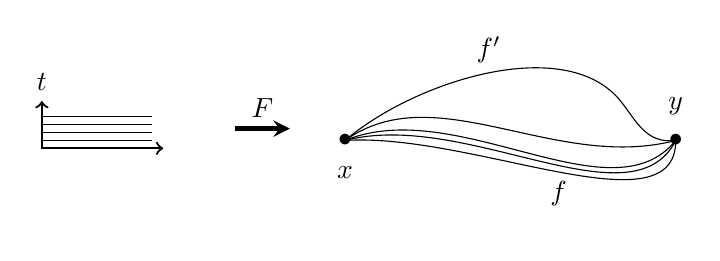
\begin{tikzpicture}[xscale=0.7, yscale=0.5]
		\draw [thick, <->] (1.5, 6.2) node [above] {$t$} -- (1.5, 5) -- (3.7, 5);
		\draw (1.5, 5.2) -- (3.5, 5.2);
		\draw (1.5, 5.4) -- (3.5, 5.4);
		\draw (1.5, 5.6) -- (3.5, 5.6);
		\draw (1.5, 5.8) -- (3.5, 5.8);

		\draw[-stealth, ultra thick] (5, 5.5) -- (6, 5.5) node[midway, above] {$F$};

		\coordinate (x) at (7, 5.2);
		\coordinate (y) at (13, 5.2);
		\node[label=below:$x$]  (x) at (7, 5.2) {$\bullet$};
		\node[label=above:$y$]  (y) at (13, 5.2) {$\bullet$};
		\draw (x.center) to [out=5, in=-90, edge node={node[below] {$f$}}] (y.center);
		\draw (x.center) to [out=20, in=-110] (y.center);
		\draw (x.center) to [out=30, in=-120] (y.center);
		\draw (x.center) to [out=45, in=-160] (y.center);
		\draw (x.center) to [out=50, in=-240, edge node={node[above] {$f'$}}]++(5, 1) to [out=-60, in=-170] (y.center);
	\end{tikzpicture}\end{center}
	空间 $X$ 的基本广群 $\Pi_1(X)$ 定义为如下范畴, 其对象是 $X$ 中的点, 对任意 $x,y \in X$, 态射集 $\Hom(x,y)$ 定义为所有从 $x$ 到 $y$ 的道路类; 态射的合成定义为道路类的合成, 而恒等态射 $\identity_x$ 由静止道路 $\forall t, \; \identity_x(t) = x$ 表之. 对于给定的态射 $f: x \to y$ (视同同伦类中的某个代表元), 其逆可以取为反向道路
	\[ f^{-1}(t) := f(1 - t), \quad 0 \leq t \leq 1. \]

	可以验证这些操作都是良定的, 并使得 $\Pi_1(X)$ 成为广群. 注意到 $\Aut(x) = \Hom(x,x)$ 正好是以 $x$ 为基点的\emph{基本群} $\pi_1(X, x)$.

	基本群是拓扑学中重要的不变量, 它为每个空间 $X$ 指定一个相应的代数结构 (群). 基本广群可以视为再高一阶的不变量: 它为 $X$ 指定一个范畴. 进一步的讨论见 \cite[Chapter 2]{May99}. 但读者应该留意到还有大量的拓扑信息被 $\Pi_1(X)$ 的范畴结构遗漏了: 除了道路的同伦类, 我们应该计入道路间的所有同伦等价, 还可以设想同伦之间更有同伦, 直至无穷. 凡此种种都必须以更高阶的范畴语言反映.
\end{example}

最后介绍一个简单而方便的概念: 反范畴.
\begin{definition}\index{fanchou!反范畴 (opposite category)}\index[sym1]{Cop@$\mathcal{C}^\text{op}$}
	对于任意范畴 $\mathcal{C}$, 其\emph{反范畴} $\mathcal{C}^\text{op}$ 定义如下:
	\begin{compactitem}
		\item $\Obj(\mathcal{C}^{\text{op}}) = \Obj(\mathcal{C})$,
		\item 对任意对象 $X, Y$, $\Hom_{\mathcal{C}^{\text{op}}}(X, Y) := \Hom_{\mathcal{C}}(Y, X)$,
		\item 态射 $f \in \Hom_{\mathcal{C}^{\text{op}}}(Y, Z)$, $g \in \Hom_{\mathcal{C}^{\text{op}}}(X, Y)$ 在 $\mathcal{C}^{\text{op}}$ 中的合成 $f \circ^\text{op} g$ 定义为 $\mathcal{C}$ 中的反向合成 $g \circ f$,
		\item 恒等态射定义同 $\mathcal{C}$.
	\end{compactitem}
\end{definition}
容易验证 $\mathcal{C}^\text{op}$ 满足范畴定义, 而且 $(\mathcal{C}^\text{op})^{\text{op}} = \mathcal{C}$. 一句话, $\mathcal{C}^\text{op}$ 的构造就是反转箭头, 反转后范畴论的公理依然成立, 范畴论中的这种对称性也称作对偶原理. 举例明之, $\mathcal{C}^\text{op}$ 中的单态射无非是 $\mathcal{C}$ 中的满态射. 在处理许多范畴论性质时, 善用对称性能省事不少.

\section{函子与自然变换}\label{sec:functors}
\begin{definition}[函子]\label{def:functor}\index{hanzi@函子 (functor)}
	设 $\mathcal{C}', \mathcal{C}$ 为范畴. 一个函子 $F: \mathcal{C}' \to \mathcal{C}$ 意谓以下资料:
	\begin{enumerate}[(i)]
		\item 对象间的映射 $F: \Obj(\mathcal{C}') \to \Obj(\mathcal{C})$.
		\item 态射间的映射 $F: \Mor(\mathcal{C}') \to \Mor(\mathcal{C})$, 使得
			\begin{compactitem}
				\item $F$ 与来源和目标映射相交换 (即 $sF=Fs$, $tF=Ft$), 等价的说法是对每个 $X, Y \in \Obj(\mathcal{C}')$ 皆有映射 $F: \Hom_{\mathcal{C}'}(X, Y) \to \Hom_{\mathcal{C}}(FX, FY)$;
				\item $F(g \circ f) = F(g) \circ F(f)$, $F(\identity_X) = \identity_{FX}$.
			\end{compactitem}
	\end{enumerate}
	对于 $F: \mathcal{C}_1 \to \mathcal{C}_2$, $G: \mathcal{C}_2 \to \mathcal{C}_3$, 合成函子 $G \circ F: \mathcal{C}_1 \to \mathcal{C}_3$ 的定义是显然的: 取合成映射
	\begin{gather*}
		\Obj(\mathcal{C}_1) \xrightarrow{F} \Obj(\mathcal{C}_2) \xrightarrow{G} \Obj(\mathcal{C}_3), \\
		\Mor(\mathcal{C}_1) \xrightarrow{F} \Mor(\mathcal{C}_2) \xrightarrow{G} \Mor(\mathcal{C}_3).
	\end{gather*}
\end{definition}
旧文献常将上述函子称为 $\mathcal{C}'$ 到 $\mathcal{C}$ 的共变函子, 而称形如 $F: (\mathcal{C}')^\text{op} \to \mathcal{C}$ 的函子为反变函子.

\begin{remark}\label{rem:op-functor}
	从 $\mathcal{C}'$ 到 $\mathcal{C}$ 和从 $(\mathcal{C}')^\text{op}$ 到 $\mathcal{C}^\text{op}$ 的函子是一回事. 为资区分, 对于函子 $F: \mathcal{C}' \to \mathcal{C}$, 反范畴间的相应函子记为 $F^\text{op}: (\mathcal{C}')^\text{op} \to \mathcal{C}^\text{op}$.
\end{remark}

\begin{definition}\index{hanzi!全 (full)}\index{hanzi!本质满 (essentially surjective)}\index{hanzi!忠实 (faithful)}
	对于函子 $F:  \mathcal{C}' \to \mathcal{C}$,
	\begin{enumerate}
		\item 称 $F$ 是本质满的, 若 $\mathcal{C}$ 中任一对象都同构于某个 $FX$;
		\item 称 $F$ 是忠实的, 若对所有 $X, Y \in \Obj(\mathcal{C}')$ 映射 $\Hom_{\mathcal{C}'}(X, Y) \to \Hom_{\mathcal{C}}(FX, FY) $ 都是单射;
		\item 称 $F$ 是全的, 如果上述映射对所有 $X, Y \in \Obj(\mathcal{C}')$ 都是满射.
	\end{enumerate}
\end{definition}

\begin{example}\label{eg:functors}
	数学中用到的函子说之不尽, 略举数端如下.
	\begin{enumerate}
		\item 子范畴 $\mathcal{C}' \subset \mathcal{C}$ 显然给出一个包含函子 $\iota: \mathcal{C}' \hookrightarrow \mathcal{C}$; 包含函子总是忠实的, 它是全函子当且仅当 $\mathcal{C}'$ 是全子范畴. 取 $\mathcal{C}' = \mathcal{C}$ 就得到恒等函子 $\identity_{\mathcal{C}}: \mathcal{C} \to \mathcal{C}$.
		\item 考虑群范畴 $\cate{Grp}$. 对于任一个群 $G$, 总是可以忘掉 $G$ 的群结构而视之为集合, 群同态当然也可以视为集合间的映射, 此程序给出\emph{忘却函子} $\cate{Grp} \to \cate{Set}$. 准此要领可对其他结构定义忘却函子, 例如 $\cate{Top} \to \cate{Set}$ (忘掉空间的拓扑结构), $\cate{Vect}(\Bbbk) \to \cate{Ab}$ (忘掉 $\Bbbk$-向量空间 $V$ 的纯量乘法, 只看它的加法群 $(V, +)$, 这里 $\Bbbk$ 是任意域) 等等, 不一一列举. 这类函子显然忠实而非全.\index{wangquehanzi@忘却函子 (forgetful functor)}
		\item 考虑域 $\Bbbk$ 上的向量空间范畴 $\cate{Vect}(\Bbbk)$. 对于任意 $\Bbbk$-向量空间 $V$, 定义其对偶空间 \index[sym1]{$V^\vee$}
			\[ V^\vee := \Hom_\Bbbk(V, \Bbbk) = \{ \Bbbk-\text{线性映射}\; V \to \Bbbk \}. \]
			任一线性映射 $f: V_1 \to V_2$ 诱导对偶空间的反向映射
			\begin{align*}
				f^\vee: V_2^\vee & \longrightarrow V_1^\vee, \\
				[\lambda: V_2 \to \Bbbk] & \longmapsto \lambda \circ f.
			\end{align*}
			易见 $D: V \mapsto V^\vee$, $f \mapsto f^\vee$ 定义了函子 $D: \cate{Vect}(\Bbbk)^\text{op} \to \cate{Vect}(\Bbbk)$, 可以验证 $D$ 是忠实的. 根据注记 \ref{rem:op-functor}, 我们有合成函子 $D D^\text{op}: \cate{Vect}(\Bbbk) \to \cate{Vect}(\Bbbk)$.
			
			将 $D$ 限制于有限维向量空间, 便得到函子 $D: \cate{Vect}_f(\Bbbk)^\text{op} \to \cate{Vect}_f(\Bbbk)$ 和 $D D^\text{op}: \cate{Vect}_f(\Bbbk) \to \cate{Vect}_f(\Bbbk)$. 分别称为对偶和双对偶函子.
		\item 对于任意群 $G$, 定义导出子群 $G_\text{der}$ 为子集 $\{xyx^{-1} y^{-1} : x,y \in G \}$ 生成的正规子群. 商群 $G/G_\text{der}$ 是交换群, 称作 $G$ 的 Abel 化 (参看引理 \ref{prop:abelianization}). 对于任意群同态 $\varphi: G \to H$, 从定义可看出 $\varphi(G_\text{der}) \subset H_\text{der}$, 因此 $\varphi$ 诱导出交换群的同态 $\bar{\varphi}: G/G_\text{der} \to H/H_\text{der}$. 容易验证 $G \mapsto G/G_\text{der}$, $\varphi \mapsto \bar{\varphi}$ 定义了 Abel 化函子 $\cate{Grp} \to \cate{Ab}$. Abel 化函子不是忠实函子.
		\item 对任意带点拓扑空间 $(X,x)$ 指定基本群 $\pi_1(X, x)$, 这就给出了函子 $\cate{Top}_\bullet \to \cate{Grp}$. 代数拓扑学中还有许多例子, 例如空间的同调群 $X \mapsto H_n(X; \Z)$ 便给出了一族函子 $H_n: \cate{Top} \to \cate{Ab}$, 其中 $n \in \Z_{\geq 0}$, 而上同调群给出函子 $H^n: \cate{Top}^\text{op} \to \cate{Ab}$.
	\end{enumerate}
\end{example}

\begin{definition}[自然变换, 或函子间的态射]\index{ziranbianhuan@自然变换 (natural transformation)}
	函子 $F, G: \mathcal{C}' \to \mathcal{C}$ 之间的自然变换 $\theta$ 是一族态射
	\[ \theta_X \in \Hom_{\mathcal{C}}(FX, GX), \quad X \in \Obj(\mathcal{C}'), \]
	使得下图对所有 $\mathcal{C}'$ 中的态射 $f: X \to Y$ 交换
	\begin{equation}\label{eqn:naturaltrans-def}\begin{tikzcd}
		FX \arrow[r, "\theta_X"] \ar[d, "Ff"'] & GX \arrow[d, "Gf"] \\
		FY \arrow[r, "\theta_Y"'] & GY .
	\end{tikzcd}\end{equation}
	上述自然变换写作 $\theta: F \to G$, 或图解为
	\[ \begin{tikzcd}
		\mathcal{C}' \arrow[bend left=50, r, "F", ""' name=U] \arrow[bend right=50, r, "G"', "" name=D] & \arrow[Rightarrow, to path=(U) -- (D) \tikztonodes, "\theta"] \mathcal{C}.
	\end{tikzcd} \]
\end{definition}
上述带有双箭头 $\Rightarrow$ 的图表有时也被称为 $2$-胞腔, 参看 \S\ref{sec:2-cat}. 一种兴许更有益的看法是设想 $\theta$ 为从 $F$ 到 $G$ 的一个同伦.

\begin{convention}\label{con:naturaltrans-morphism}\index{ziran@自然}\index{dianfan@典范}
	我们也将自然变换 $\theta: F \to G$ 称为从函子 $F$ 到 $G$ 的态射. 实用中经常会省略严格的范畴论框架, 只说态射 $\theta_X: FX \to GX$ 对于变元 $X$ 是\emph{自然}的, \emph{典范}的, 或称满足\emph{函子性}. 实践中经常把自然同构直接写成等号 $=$.
\end{convention}

接着介绍自然变换的几种操作, 包括纵, 横两种合成.\index{ziranbianhuan!合成}
\begin{itemize}
	\item 考虑 $\mathcal{C}'$ 到 $\mathcal{C}$ 的三个函子间的态射 $\theta: F \to  G$,  $\psi: G \to H$. 纵合成 $\psi \circ \theta$ 的定义是 $\{ \psi_X \circ \theta_X : X \in \Obj(\mathcal{C}') \}$, 图解:
	\[\begin{tikzcd}
		\mathcal{C}'
			\arrow[bend left=70, rr, "F", ""' name=U]
			\arrow[rr, "G" name=MM, ""' name=M]
			\arrow[bend right=70, rr, "" name=D, "H"'] & &
		\arrow[Rightarrow, to path=(U) -- (MM) \tikztonodes, "\theta"] \arrow[Rightarrow, to path=(M) -- (D) \tikztonodes, "\psi"] \mathcal{C} 
	\end{tikzcd} \quad \text{合成为} \quad \begin{tikzcd}
		\mathcal{C}'
		\arrow[bend left=50, rr, "F", ""' name=U]
		\arrow[bend right=50, rr, "" name=D, "H"']
		& & \arrow[Rightarrow, to path=(U) -- (D) \tikztonodes, "\psi \circ \theta"] \mathcal{C} .
	\end{tikzcd}\]
	\item 考虑函子
	$\begin{tikzcd}
		\mathcal{C}'' \arrow[bend left=30, r, "F_1"] \arrow[bend right=30, r, "F_2"] & \mathcal{C}' \arrow[bend left=30, r, "G_1"] \arrow[bend right=30, r, "G_2"] & \mathcal{C}
	\end{tikzcd}$
	及态射 $\theta: F_1 \to F_2$, $\psi: G_1 \to G_2$. 今将定义横合成 $\psi \circ \theta: G_1 \circ F_1 \to G_2 \circ F_2$. 首先注意到对所有 $X \in \Obj(\mathcal{C}'')$, 根据 $\psi$ 的自然性, 图表
	\begin{equation}\label{eqn:horizontal-comp}\begin{tikzcd}
		G_1 F_1(X) \arrow[r, "{\psi_{F_1 X}}"] \arrow[d, "{G_1(\theta_X)}"'] & G_2 F_1(X) \arrow[d, "{G_2(\theta_X)}"] \\
		G_1 F_2(X) \arrow[r, "{\psi_{F_2 X}}"'] & G_2 F_2(X)
	\end{tikzcd}\end{equation}
	交换. 对角合成 $\searrow$ 记作 $(\psi \circ \theta)_X : G_1 F_1 (X) \to G_2 F_2 (X)$, 此即所求的横合成, 我们马上会证明它的自然性, 读者也可以借机熟悉交换图表的运用. 图解:
	\[ \begin{tikzcd}
		\mathcal{C}'' \arrow[bend left=50, r, "F_1", ""' name=LU] \arrow[bend right=50, r, "" name=LD, "F_2"'] &
		\mathcal{C}' \arrow[bend left=50, r, "G_1", ""' name=RU] \arrow[bend right=50, r, "" name=RD, "G_2"'] &
		\arrow[Rightarrow, to path=(LU) -- (LD) \tikztonodes, "\theta"] \arrow[Rightarrow, to path=(RU) -- (RD) \tikztonodes, "\psi"] \mathcal{C}
	\end{tikzcd} \quad \text{合成为} \quad \begin{tikzcd}
		\mathcal{C}''
		\arrow[bend left=50, rr, "G_1 F_1", ""' name=U]
		\arrow[bend right=50, rr, "" name=D, "G_2 F_2"']
		& & \arrow[Rightarrow, to path=(U) -- (D) \tikztonodes, "\psi \circ \theta"] \mathcal{C} .
	\end{tikzcd} \]
	\item 横合成有下述特例. 请端详
	\[\begin{tikzcd}
		\mathcal{C}_1 \arrow[r, "H"] & \mathcal{C}_2 \arrow[bend left=50, r, "F", ""' name=U] \arrow[bend right=50, r, "" name=D, "G"'] & \mathcal{C}_3 \arrow[Rightarrow, to path=(U)--(D) \tikztonodes, "\theta"] \arrow[r, "K"] & \mathcal{C}_4 .
    \end{tikzcd} \]
	先看左边三项: 我们将以 $\theta H: FH \to GH$ 简记横合成 $\theta \circ \identity_{H}$; 具体地说, $(\theta H)_X = \theta_{HX} : FH(X) \to GH(X)$; 类似地处理右三项: 记 $K\theta: KF \to KG$ 为横合成 $\identity_K \circ \theta$, 我们有 $(K\theta)_X = K(\theta_X): KF(X) \to KG(X)$.
\end{itemize}
注意到我们用同一个符号 $\circ$ 表示纵横合成, 如有混淆之虞将另作说明.

\begin{lemma}\label{prop:naturaltrans-associativity}
	以上定义的纵, 横合成 $\{ (\psi \circ \theta)_X \}_X$ 都是函子间的态射, 而且各自满足严格结合律 $(\phi \circ \psi) \circ \theta = \phi \circ (\psi \circ \theta)$. 纵横合成之间满足下述关系: 对于图表
	\[\begin{tikzcd}
		\mathcal{C}_1
		\arrow[bend left=70, rr, ""' name=U]
		\arrow[rr, "" name=MM, ""' name=M]
		\arrow[bend right=70, rr, "" name=D] & &
		\arrow[Rightarrow, to path=(U) -- (MM) \tikztonodes, "\theta"] \arrow[Rightarrow, to path=  (M) -- (D) \tikztonodes, "\psi"] \mathcal{C}_2
		\arrow[bend left=70, rr, ""' name=V]
		\arrow[rr, "" name=NN, ""' name=N]
		\arrow[bend right=70, rr, "" name=E] & &
		\arrow[Rightarrow, to path=(V) -- (NN) \tikztonodes, "\theta'"] \arrow[Rightarrow, to path=  (N) -- (E) \tikztonodes, "\psi'"] \mathcal{C}_3 ,
	\end{tikzcd} \]
	以下的互换律成立
	\[ \left( \psi' \underset{\text{纵}}{\circ} \theta'\right) \underset{\text{横}}{\circ} \left( \psi \underset{\text{纵}}{\circ} \theta\right) = \left( \psi' \underset{\text{横}}{\circ} \psi \right) \underset{\text{纵}}{\circ} \left( \theta' \underset{\text{横}}{\circ} \theta\right).  \]
\end{lemma}
\begin{proof}
	关于纵合成的断言是简单的, 以下证明横合成是函子间的态射. 我们沿用之前的符号. 对于 $\mathcal{C}''$ 中的态射 $f: X \to Y$, 考虑源于 \eqref{eqn:horizontal-comp} 的图表
	\[\begin{tikzcd}
		G_1 F_1 (X) \arrow[r, "G_1 \theta_X"] \arrow[d, "G_1 F_1 f"'] & G_1 F_2 (X) \arrow[r, "{\psi_{F_2 X}}"] \arrow[d, "G_1 F_2 f"] & G_2 F_2 (X) \arrow[d, "G_2 F_2 f"] \\
		G_1 F_1 (Y) \arrow[r, "{G_1 \theta_Y}"'] & G_1 F_2 (Y) \arrow[r, "{\psi_{F_2 Y}}"'] & G_2 F_2 (Y) .
	\end{tikzcd} \]
	按定义, 水平方向箭头合成后上下分别是 $(\psi \circ \theta)_X$ 和 $(\psi \circ \theta)_Y$. 因为 $\theta$ 是自然变换而 $G_1$ 是函子, 左方块交换; 由于 $\psi$ 是自然变换, 右方块交换. 将箭头分段作合成, 可知整个大方块交换, 此即 $ \psi \circ \theta$ 所需性质.

	现证明横合成的结合律: 考虑函子间的态射
	\[\begin{tikzcd}
		\mathcal{C}''' \arrow[bend left=50, r, "F_1", ""' name=LU] \arrow[bend right=50, r, "" name=LD, "F_2"'] &
		\mathcal{C}'' \arrow[bend left=50, r, "G_1", ""' name=MU] \arrow[bend right=50, r, "" name=MD, "G_2"'] &
		\mathcal{C}' \arrow[bend left=50, r, "H_1", ""' name=RU] \arrow[bend right=50, r, "" name=RD, "H_2"'] &
		\arrow[Rightarrow, to path=(LU) -- (LD) \tikztonodes, "\theta"]
		\arrow[Rightarrow, to path=(MU) -- (MD) \tikztonodes, "\psi"]
		\arrow[Rightarrow, to path=(RU) -- (RD) \tikztonodes, "\phi"]
		\mathcal{C} .
	\end{tikzcd} \]
	对任意 $X \in \Obj(\mathcal{C}''')$, 考虑图表
	\[\begin{tikzcd}[row sep=small]
		& & H_1 G_2 F_2(X) \arrow[rd] & \\
		H_1 G_1 F_1(X) \arrow[r] & H_1 G_2 F_1(X) \arrow[ru] \arrow[rd] & & H_2 G_2 F_2(X) . \\
		& & H_2 G_2 F_1(X) \arrow[ru] &
	\end{tikzcd}\]
	施 $\phi$ 的自然性于 $G_2 F_1(X) \to G_2 F_2(X)$ 可知菱形部分交换. 按
	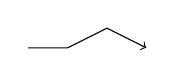
\begin{tikzpicture}[scale=0.5, baseline=(X)]
		\draw[->] (0,0) -- (1,0) -- (2, 0.5) -- (3, 0);
		\coordinate (X) at (0,0);
	\end{tikzpicture}
	合成给出 $(\phi \circ (\psi \circ \theta))_X$. 按
	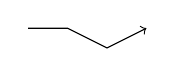
\begin{tikzpicture}[scale=0.5, baseline=(X)]
		\draw[->] (0,0) -- (1,0) -- (2, -0.5) -- (3, 0);
		\coordinate (X) at (0, -0.2);
	\end{tikzpicture}
	合成则给出 $((\phi \circ \psi) \circ \theta)_X$; 这里仍须用上交换图表 \eqref{eqn:horizontal-comp}. 结合律证毕.

	最后一个等式可以同样按图索骥, 细节交给感兴趣的读者.
\end{proof}

任意函子 $F$ 到自身有恒等态射 $\identity_F : F \to F$. 给定函子间的态射 $\theta: F_1 \to F_2$, 若态射 $\psi: F_2 \to F_1$ 满足 $\psi \circ \theta = \identity_{F_1}$, $\theta \circ \psi = \identity_{F_2}$, 则称 $\psi$ 是 $\theta$ 的逆. 可逆的态射称为函子间的同构, 写作 $\theta: F_1 \rightiso F_2$. 由定义直接看出 $\theta$ 的逆若存在则是唯一的, 记作 $\theta^{-1}$, 它无非是在范畴中``逐点地''取逆: $(\theta^{-1})_X := (\theta_X)^{-1}: F_2 X \rightiso F_1 X$. 同理可见态射 $\theta$ 可逆当且仅当每个 $\theta_X$ 都可逆. 易见同构的纵横合成仍是同构. 函子间同构 $\theta: F_1 \rightiso F_2$ 的等价说法是称 $\theta_X: F_1 X \rightiso F_2 X$ 对变元 $X$ 是\emph{自然同构}或\emph{典范同构}.

\begin{definition}[等价]\label{def:cat-equivalence}\index{fanchoudengjia@范畴等价 (equivalence)}\index{hanzi!拟逆 (quasi-inverse)}
	如果一对函子
	\begin{tikzcd}
		\mathcal{C}_1 \arrow[bend left=20, r, "F"] & \mathcal{C}_2 \arrow[bend left=20, l, "G"]
	\end{tikzcd}
	满足以下性质: 存在函子之间的同构 $\theta: FG \rightiso \identity_{\mathcal{C}_2}$, $\psi: GF \rightiso \identity_{\mathcal{C}_1}$, 则称 $G$ 是 $F$ 的\emph{拟逆函子}, 并称 $F$ 是范畴 $\mathcal{C}_1$ 到 $\mathcal{C}_2$ 的\emph{等价}.

	如果进一步有 $FG = \identity_{\mathcal{C}_2}$, $GF = \identity_{\mathcal{C}_1}$, 则称 $F$ 是范畴间的\emph{同构}, 而 $G$ 是 $F$ 的\emph{逆}.
\end{definition}
容易证明等价的合成仍是等价, 细节留作习题.

\begin{example}
	令 $\cate{CHaus}$ 为紧 Hausdorff 拓扑空间范畴, $C^*\dcate{CommAlg}$ 为含幺元的交换 $C^*$-代数所成范畴 (态射为保幺元的 $\ast$-同态). 交换版本的 Gelfand--Naimark 定理断言函子
	\[ \begin{tikzcd}[row sep=tiny]
		\cate{CHaus}^{\text{op}} \arrow[yshift=0.7ex]{r} & C^*\dcate{CommAlg} \arrow[yshift=-0.7ex]{l} \\
		X \arrow[mapsto]{r} & C(X): \text{连续复值函数空间} \\
		\mathfrak{M}_A: \text{ 极大理想空间} & A \arrow[mapsto]{l}
	\end{tikzcd} \]
	互为拟逆:  Gelfand 变换 $a \mapsto \hat{a}$ 给出自然同构 $A \rightiso C(\mathfrak{M}_A)$, 可参看 \cite[定理 5.4.8]{Zh2}; 反向的自然同构 $X \rightiso \mathfrak{M}_{C(X)}$ 相对容易, 参看 \cite[定理 5.3.2]{Zh2}.
\end{example}

\begin{proposition}
	若 $G, G'$ 是函子 $F: \mathcal{C}_1 \to \mathcal{C}_2$ 的拟逆, 则存在函子的同构 $G \simeq G'$.
\end{proposition}
\begin{proof}
	自然变换的横合成给出 $G \xleftarrow[\sim]{\psi' \circ \identity_G} (G'F)G = G'(FG) \xrightarrow[\sim]{\identity_{G'} \circ \theta} G'$.
\end{proof}

\begin{remark}\label{rem:strict-or-not}
	我们业已对对象间的态射和函子间的态射 (自然变换) 定义了逆的概念, 其逆若存在则唯一, 依此定义何谓对象间或函子间的同构. 对于函子亦可定义逆的概念, 逆函子若存在则唯一; 相较之下, 拟逆函子之间则可以差一个同构. 实践表明范畴的同构概念不甚实用, 等价的概念则处处出现. 这体现了范畴论的一条经验准则: 在函子层次, 同构 (如之前的 $\theta: FG \rightiso \identity$) 几乎总是比严格相等 (如之前的 $FG = \identity$) 来得管用. 然而同构也不是任意的, 所需的条件一般称为融贯性: 以等价为例, 读者兴许已经在先前论证中感到拟逆的概念有些松散, 定理 \ref{prop:adjoint-equivalence} 将给出称为\emph{伴随等价}的一种细化. \index{bansuidengjia@伴随等价 (adjoint equivalence)}
\end{remark}

称一个全子范畴 $\mathcal{C}' \subset \mathcal{C}$ 是 $\mathcal{C}$ 的一副\emph{骨架}, 如果对 $\mathcal{C}$ 的每个对象 $X$ 都存在同构 $X \rightiso Y \in \Obj(\mathcal{C}')$, 而且此 $Y \in \Obj(\mathcal{C}')$ 是唯一的. 自为骨架的范畴称为\emph{骨架范畴}.\index{fanchou!骨架 (skeleton)}

\begin{lemma}\label{prop:skeletal-cat-isom}
	任意范畴 $\mathcal{C}$ 总有一副骨架 $\mathcal{C}'$, 而且包含函子 $\iota: \mathcal{C}' \hookrightarrow \mathcal{C}$ 是等价. 骨架范畴间的全忠实, 本质满函子都是同构.
\end{lemma}
\begin{proof}
	先证第一部分. 以选择公理在 $\Obj(\mathcal{C})$ 的每个同构类中选定代表元, 由这些代表元构成的全子范畴记作 $\mathcal{C}'$. 同理, 对每个 $X \in \Obj(\mathcal{C})$ 可以选定同构 $\theta_X: X \rightiso \kappa(X) $, 其中 $\kappa(X) \in \Obj(\mathcal{C}')$; 不妨假设对于 $X \in \Obj(\mathcal{C}')$ 有 $\theta_X = \identity_X$. 存在唯一一种方法将 $\kappa: \Obj(\mathcal{C}) \to \Obj(\mathcal{C}')$ 延拓为函子并使得 $\theta: \identity_{\mathcal{C}} \rightiso \iota \kappa$: 置
	\[ \kappa(f) := \theta_Y \circ f \circ \theta_X^{-1} \in \Hom_{\mathcal{C}'}(\kappa(X), \kappa(Y)), \quad f \in \Hom_{\mathcal{C}}(X, Y). \]
	另一方面, 我们有函子的等式 $\kappa\iota = \identity_{\mathcal{C}'}$. 因此 $\kappa$ 是 $\iota$ 的拟逆函子.
	
	对于第二部分, 设 $F: \mathcal{C}_1 \to \mathcal{C}_2$ 是骨架范畴间的全忠实, 本质满函子. 对任意 $\mathcal{C}_2$ 中对象 $Z$, 存在 $X$ 使得 $Z \simeq FX$, 因此 $Z = FX$. 这样的 $X$ 是唯一的, 因为全忠实性和 $FX \simeq FX'$ 蕴涵 $X \simeq X'$. 于是 $F$ 在对象集上是双射, 由此可定义其逆函子 $G$.
\end{proof}

\begin{theorem}\label{prop:functor-equiv-criterion}\index{fanchoudengjia}
	对于函子 $F: \mathcal{C}_1 \to \mathcal{C}_2$, 以下叙述等价.
	\begin{compactenum}
		\item $F$ 是范畴等价,
		\item $F$ 是全忠实, 本质满函子.
	\end{compactenum}
\end{theorem}
\begin{proof}
	假设 $F$ 是范畴等价, 取拟逆函子 $G: \mathcal{C}_2 \to \mathcal{C}_1$ 和 $GF \xrightarrow[\sim]{\psi} \identity_{\mathcal{C}_1}$, $FG \xrightarrow[\sim]{\phi} \identity_{\mathcal{C}_2}$. 对 $\mathcal{C}_2$ 中任何对象 $Z$ 都有 $\phi_Z: F(GZ) \rightiso Z$ 故 $F$ 本质满, 同理 $G$ 本质满. 观察到
	\[\begin{tikzcd}[row sep=tiny, column sep=small]
		\Hom(X,Y) \arrow[r, "F"] & \Hom(FX, FY) \arrow[r, "G"] & \Hom(GF(X), GF(Y)) \arrow[r, "\sim"] & \Hom(X, Y) \\
		f \arrow[mapsto, r] & Ff \arrow[mapsto, r] & GF(f) \arrow[mapsto, r] & \psi_Y GF(f) \psi_X^{-1}
	\end{tikzcd}\]
	合成为恒等映射, 故图中第一个箭头 $F$ 左可逆, 第二个箭头 $G$ 右可逆. 调换 $F, G$ 的角色可知当 $X, Y \in \Obj(\mathcal{C}_1)$ 属于 $G$ 的像时, $\Hom(X, Y) \xrightarrow{F} \Hom(FX, FY)$ 右可逆. 然而 $\mathcal{C}_1$ 中每个对象都同构于 $G$ 的某个像, 综之 $F$ 是全忠实函子.

	现证反向断言. 以引理 \ref{prop:skeletal-cat-isom} 取骨架 $\iota_i: \mathcal{C}'_i \rightarrow \mathcal{C}_i$ 及其拟逆函子 $\kappa_i$ (此处 $i=1,2$). 函子 $F' := \kappa_2 \circ F \circ \iota_1: \mathcal{C}'_1 \to \mathcal{C}'_2$ 仍是全忠实本质满函子, 因而知 $F'$ 是范畴的同构. 设 $G := \iota_1 \circ F'^{-1} \circ \kappa_2$, 则
	\begin{gather*}
		GF = \iota_1  F'^{-1} \kappa_2 F \simeq \iota_1  F'^{-1} \underbracket{\kappa_2 F \iota_1}_{= F'} \kappa_1 = \iota_1 \kappa_1 \simeq \identity_{\mathcal{C}_1}, \\
		FG = F \iota_1  F'^{-1} \kappa_2 \simeq \iota_2 \underbracket{\kappa_2 F \iota_1}_{= F'}  F'^{-1} \kappa_2 = \iota_2 \kappa_2 \simeq \identity_{\mathcal{C}_2}.
	\end{gather*}
	这里用到了自然变换的横合成.
\end{proof}

\begin{example}\label{eg:vectf-duality}
	继续考虑某域 $\Bbbk$ 上的向量空间范畴 $\cate{Vect}(\Bbbk)$ 及其子范畴 $\cate{Vect}_f(\Bbbk)$. 在例 \ref{eg:functors} 中已定义了双对偶函子 $D D^\text{op}: \cate{Vect}(\Bbbk) \to \cate{Vect}(\Bbbk)$. 对于任意向量空间 $V$ 皆有求值映射
	\begin{align*}
		\text{ev}: V & \longrightarrow DD^\text{op} V = (V^\vee)^\vee \\
		v & \longmapsto [\lambda \mapsto \lambda(v)].
	\end{align*}
	对于任意线性映射 $f: V \to W$, 从 $f^\vee$ 的定义不难检查以下图表
	\[\begin{tikzcd}
		V \arrow[r, "\text{ev}"] \ar[d, "f"'] & DD^\text{op} V \arrow[d, "{DD^\text{op} f}"] \\
		W \ar[r, "\text{ev}"'] & DD^\text{op} W
	\end{tikzcd} \]
	是交换的, 于是有 $\text{ev}: \identity \to D D^\text{op}$. 容易看出 $\text{ev}: V \to D D^\text{op} V$ 总是单射, 事实上可以证明 $\text{ev}$ 是双射当且仅当 $V$ 有限维. 一切限制到全子范畴 $\cate{Vect}_f(\Bbbk)$ 上, 遂有同构
	\[ \text{ev}: \identity_{\cate{Vect}_f(\Bbbk)} \rightiso D D^\text{op}. \]
	同一式子在相反范畴中诠释, 便是
	\[ \identity_{\cate{Vect}_f(\Bbbk)^\text{op}} \rightiso D^\text{op} D. \]
	故函子 $D: \cate{Vect}_f(\Bbbk)^\text{op} \to \cate{Vect}_f(\Bbbk)$ 是范畴间的等价, 而 $D^\text{op}: \cate{Vect}_f(\Bbbk) \to \cate{Vect}_f(\Bbbk)^\text{op}$ 则是它的拟逆.
\end{example}

\begin{example}
	选定域 $\Bbbk$, 定义范畴 $\cate{Mat}$ 如下: 其对象是 $\Z_{\geq 0}$, 对任意对象 $n, m \in \Z_{\geq 0}$, 定义 $\Hom(n, m) := M_{m \times n}(\Bbbk)$ 为域 $\Bbbk$ 上的全体 $m \times n$ 矩阵 $A = (a_{ij})_{\substack{1 \leq i \leq m \\ 1 \leq j \leq n}}$ 所成集合. 约定 $M_{0 \times n}(\Bbbk) = M_{m \times 0}(\Bbbk) := \{0\}$. 态射的合成定义为寻常的矩阵乘法
	\begin{align*}
		\Hom(n, m) \times \Hom(m, k) & \longrightarrow \Hom(n, k) \\
		(A, B) & \longmapsto BA .
	\end{align*}

	定义函子 $F: \cate{Mat} \to \cate{Vect}_f(\Bbbk)$ 如下: 置 $F(n) = \Bbbk^{\oplus n} := M_{n \times 1}(\Bbbk)$, 而对 $A \in \Hom(n, m)$, 线性映射 $FA: \Bbbk^{\oplus n} \to \Bbbk^{\oplus m}$ 是矩阵乘法 $v \mapsto Av$. 我们断言 $F$ 是范畴等价.

	这一切只是虚张声势的线性代数. 首先留意到 $F: \Hom(n, m) \to \Hom_\Bbbk(\Bbbk^{\oplus n}, \Bbbk^{\oplus m})$ 是双射, 这无非是线性映射的矩阵表达. 再者, 从 $V \simeq \Bbbk^{\oplus \dim V}$ ($V$ 是 $\Bbbk$-向量空间) 可知 $F$ 是全忠实本质满的, 由定理 \ref{prop:functor-equiv-criterion} 可知它是范畴等价.
\end{example}

\section{函子范畴}\label{sec:functor-category}
首先对范畴定义积和余积(又称无交并)的概念, 这对陈述一些范畴性质格外有用.

回顾约定 \ref{con:U-small}: 除非另作说明, 以下所论的范畴都是 $\mathcal{U}$-范畴, 这里 $\mathcal{U}$ 是选定的宇宙. 属于 $\mathcal{U}$ 的集合称为 $\mathcal{U}$-集.

\begin{definition}\index{fanchou!积, 余积}
	设 $I$ 为 $\mathcal{U}$-集, 而 $\{\mathcal{C}_i : i \in I \}$ 是一族范畴.
	\begin{itemize}
		\item 积范畴 $\prod_{i \in I} \mathcal{C}_i$ 定义如下:
			\begin{align*}
				\Obj\left( \prod_{i \in I} \mathcal{C}_i \right) & := \prod_{i \in I} \Obj(\mathcal{C}_i), \\
				\Hom_{\prod_{i \in I} \mathcal{C}_i}( (X_i)_i, (Y_i)_i ) & := \prod_{i \in I} \Hom_{\mathcal{C}_i}(X_i, Y_i),
			\end{align*}
			其中我们以 $(X_i)_i$ 表示 $\prod_{i \in I} \Obj(\mathcal{C}_i)$ 的元素. 态射的合成是逐个分量定义的.
		\item 余积(又称无交并)范畴 $\coprod_{i \in I} \mathcal{C}_i$ 定义如下:
			\begin{align*}
				\Obj\left( \coprod_{i \in I} \mathcal{C}_i \right) & := \coprod_{i \in I} \Obj(\mathcal{C}_i), \\
				\Hom_{\coprod_{i \in I} \mathcal{C}_i}(X_j, X'_k) & :=
				\begin{cases}
					\Hom_{\mathcal{C}_j}(X_j, X'_k), & j = k, \\
					\emptyset, & j \neq k;
				\end{cases}
			\end{align*}
			其中对每个 $j \in I$, $X_j, X'_j \in \Obj(\mathcal{C}_j)$. 态射的合成是在各个 $\mathcal{C}_i$ 中个别定义的.
	\end{itemize}
\end{definition}
由于 $I$ 已假设是 $\mathcal{U}$-集, 我们造出的范畴仍然是 $\mathcal{U}$-范畴; 如果每个 $\mathcal{C}_i$ 都是 $\mathcal{U}$-小范畴, 则它们的积和余积亦然.

我们有一族投影函子 $\pr_j: \prod_{i \in I} \mathcal{C}_i \to \mathcal{C}_j$, 它将 $(X_i)_i$ 映至 $X_j$, 在态射层面也是类似地投影到 $j$ 分量. 同理定义一族包含函子 $\iota_j: \mathcal{C}_j \to \coprod_{i \in I} \mathcal{C}_i$, 将 $\mathcal{C}_j$ 以自明的方式嵌入为全子范畴.

特别地, 取 $I$ 为有限集便能定义 $\mathcal{C}_1 \times \cdots \times \mathcal{C}_n$ 和 $\mathcal{C}_1 \sqcup \cdots \sqcup \mathcal{C}_n$.

\begin{definition}
	形如 $F: \mathcal{C}_1 \times \mathcal{C}_2 \to \mathcal{C}$ 的函子称为二元函子. 多元函子 $\mathcal{C}_1 \times \cdots \times \mathcal{C}_n \to \mathcal{C}$ 的定义类似.
\end{definition}

\begin{example}[$\Hom$ 函子]\label{eg:Hom-functor} \index[sym1]{HomC}
	给定范畴 $\mathcal{C}$, 则 $(X,Y) \mapsto \Hom_{\mathcal{C}}(X, Y)$ 定义了二元函子
	\[ \Hom_{\mathcal{C}}: \mathcal{C}^\text{op} \times \mathcal{C}  \to \cate{Set}. \]
	诚然, $\mathcal{C}$ 中的任一对态射 $f: X' \to X$, $g: Y \to Y'$ 诱导出
	\begin{align*}
		\Hom_{\mathcal{C}}(X, Y) & \longrightarrow \Hom_{\mathcal{C}}(X', Y') \\
		\phi & \longmapsto g \phi f .
	\end{align*}
	有时也说这是态射 $\phi$ 对 $f$ 作\emph{拉回}, 对 $g$ 作\emph{推出}. 拉回与推出习惯用符号 $f^* \phi = \phi f$ 和 $g_* \phi = g\phi$ 表示.\index{lahui@拉回 (pullback)}\index{tuichu@推出 (pushout)}\index[sym1]{$f_*, f^*$}
	易见 $(f_1 f_2)^* = f_2^* f_1^*$ 和 $(f_1 f_2)_* = (f_1)_* (f_2)_*$.
\end{example}

\begin{definition}[函子范畴]\index{hanzifanchou@函子范畴 (functor category)}\index[sym1]{Fct@$\text{Fct}$}
	设 $\mathcal{C}_1, \mathcal{C}_2$ 为 $\mathcal{U}$-范畴, 定义函子范畴 $\text{Fct}(\mathcal{C}_1, \mathcal{C}_2)$: 其对象是 $\mathcal{C}_1$ 到 $\mathcal{C}_2$ 的函子, 任两个对象 $F, G$间的态射是自然变换 $\theta: F \to G$; 态射 $\theta: F \to G$ 与 $\psi: G \to H$ 的合成是自然变换的纵合成 $\psi \circ \theta: F \to H$.
\end{definition}
此构造解释了约定 \ref{con:naturaltrans-morphism}.

\begin{remark}
	此定义需要一些解释. 首先注意到 $\text{Fct}(\mathcal{C}_1, \mathcal{C}_2)$ 的对象和态射都构成集合. 对于态射还有更精确的结果: 若 $\mathcal{C}_1$ 是 $\mathcal{U}$-小范畴, 则 $\text{Fct}(\mathcal{C}_1, \mathcal{C}_2)$ 是 $\mathcal{U}$-范畴, 这是因为对任两个 $F, G: \mathcal{C}_1 \to \mathcal{C}_2$, 其间的自然变换是集合
	\[ \prod_{X \in \Obj(\mathcal{C}_1)} \Hom_{\mathcal{C}_2} (FX, GX) \]
	的子集. 若 $\mathcal{C}_1$ 是 $\mathcal{U}$-小范畴, 则上式为 $\mathcal{U}$-小集.

	此外还要用到自然变换纵合成的结合律, 见引理 \ref{prop:naturaltrans-associativity}.
\end{remark}

对函子 $F, G : \mathcal{C}_1 \to \mathcal{C}_2$, 在反范畴中相应地有 $F^\text{op}, G^\text{op}: \mathcal{C}_1^\text{op} \to \mathcal{C}_2^\text{op}$ (见注记 \ref{rem:op-functor}), 易见自然变换 $\varphi: F \to G$ 在反范畴中被倒转为 $\varphi^\text{op}: G^\text{op} \to F^\text{op}$, 而且 $(\varphi^{\text{op}})^{\text{op}} = \varphi$.  摘要如下.

\begin{proposition}\label{prop:op-functor-cat}
	存在自然同构 $\text{Fct}(\mathcal{C}_1, \mathcal{C}_2)^\text{op} \rightiso \text{Fct}(\mathcal{C}_1^{\text{op}}, \mathcal{C}_2^{\text{op}})$, 它将 $\varphi$ 映至 $\varphi^\text{op}$. 
\end{proposition}

今后用到的多数是 $\mathcal{C}_1$ 为小范畴的情形. 有时也把 $\text{Fct}(\mathcal{C}_1, \mathcal{C}_2)$ 写作 $\mathcal{C}_2^{\mathcal{C}_1}$.
\begin{example}
	考虑集合 $I \in \mathcal{U}$, 取 $\mathcal{I} := \cate{Disc}(I)$ 为相应的离散范畴 (例 \ref{eg:categories}), 则对任意 $\mathcal{C}$ 皆有范畴同构 $\mathcal{C}^{\mathcal{I}} \simeq \prod_{i \in I} \mathcal{C}$.
\end{example}

既定义了函子范畴, 其中自然可以讨论一个函子 $F: \mathcal{C}_1 \to \mathcal{C}_2$ 的自同态幺半群 $\End(F)$ 与自同构群 $\Aut(F)$. 它们作为集合未必属于 $\mathcal{U}$.
\begin{definition}\label{def:cat-center}\index{zhongxin@中心 (center)}
	一个范畴 $\mathcal{C}$ 的\emph{中心}定义为 $Z(\mathcal{C}) := \End(\identity_{\mathcal{C}})$.
\end{definition}

中心是范畴的一种极有用的不变量. 由 \eqref{eqn:naturaltrans-def} 可知 $Z(\mathcal{C})$ 的元素无非是一族自同态 $\psi_X: X \to X$, 使得图表
\begin{tikzcd}
	X \arrow[r, "{\psi_X}"] \arrow[d, "f"'] & X \arrow[d, "f"] \\
	Y \arrow[r, "{\psi_Y}"'] & Y
\end{tikzcd}
对每个 $f: X \to Y$ 都交换.

\begin{proposition}
	中心 $Z(\mathcal{C})$ 对二元运算 $\circ$ 总是交换的.
\end{proposition}
\begin{proof}
	对给定的 $\theta, \psi \in \End(\identity_{\mathcal{C}})$, 上图中取自同态 $\theta$, 对象 $X=Y$ 和态射$f = \psi_X$ 便得到 $\theta_X \psi_X = \psi_X \theta_X$.
\end{proof}

\begin{proposition}
	范畴等价 $F: \mathcal{C}_1 \to \mathcal{C}_2$ 诱导中心的同构 $Z(\mathcal{C}_1) \simeq Z(\mathcal{C}_2)$.
\end{proposition}
证明是容易的, 留作练习.

\section{泛性质}\label{sec:cat-universals}
许多数学构造能以泛性质唯一地刻画. 我们使用始, 终对象和逗号范畴的语言予以阐述.

\begin{definition}\label{def:universal-objects}\index{duixiang!始对象/终对象/零对象 (initial/terminal/zero object)}
	范畴 $\mathcal{C}$ 中的对象 $X$ 称为\emph{始对象}, 如果对所有对象 $Y$ 集合 $\Hom_{\mathcal{C}}(X, Y)$ 恰有一个元素. 类似地, 称 $X$ 为\emph{终对象}, 如果对所有对象 $Y$ 集合 $\Hom_{\mathcal{C}}(Y, X)$ 恰有一个元素. 若 $X$ 既是始对象又是终对象, 则称之为\emph{零对象}.
\end{definition}

始, 终对象是相互对偶的概念: $\mathcal{C}$ 的始对象无非是 $\mathcal{C}^\text{op}$ 的终对象, 反之亦然.

\begin{proposition}\label{prop:initial-obj-uniqueness}
	设 $X, X'$ 为 $\mathcal{C}$ 中的始对象, 则存在唯一的同构 $X \rightiso X'$. 同样性质对终对象也成立.
\end{proposition}
\begin{proof}
	仅需处理始对象情形. 假设 $X, X'$ 都是始对象, 则存在唯一的态射 $f: X \to X'$ 和 $g: X' \to X$. 其合成 $gf: X \to X$ 也是唯一的, 它只能是 $\identity_X$; 同理 $fg = \identity_{X'}$. 因此 $f: X \rightiso X'$ 即所求.
\end{proof}

\begin{definition}\label{def:zero-morphism}\index{taishe!零态射 (zero morphism)}
	设 $\mathcal{C}$ 中有零对象, 记作 $0$. 对任意 $X, Y \in \Obj(\mathcal{C})$ 定义\emph{零态射} $0: X \to Y$ 为
	\[ X \to 0 \to Y \]
	的合成.
\end{definition}

两点观察: (1) 零态射从左右合成任何态射仍是零态射. (2) 零态射的定义无关零对象的选取: 若 $0, 0'$ 都是零对象, 则出入 $0, 0'$ 的箭头都是唯一的, 下图自动交换
\[ \begin{tikzcd}[row sep=small]
	{} & 0 \arrow[rd] \arrow[dd, "\simeq"] & {} \\
	X \arrow[ru] \arrow[rd] & & Y . \\
	& 0' \arrow[ru] &
\end{tikzcd} \]

\begin{example}
	一般而言, 始对象和终对象未必存在 (例: 考虑离散范畴). 以下是一些典型例子:
	\begin{enumerate}
		\item 集合范畴 $\cate{Set}$: $\emptyset$ 是始对象, $\{\text{pt}\}$ 是终对象;
		\item 带基点的集合范畴 $\cate{Set}_\bullet$: $(\{\text{pt}\}, \text{pt})$ 是零对象;
		\item 群范畴 $\cate{Grp}$: 平凡群 $\{1\}$ 是零对象, 取常值 $1$ 的同态是零态射;
		\item 域 $\Bbbk$ 上的向量空间范畴 $\cate{Vect}(\Bbbk)$: 零空间是零对象, 零映射是零态射.
	\end{enumerate}
\end{example}

始, 终对象及其唯一性一般被用来表述\emph{泛性质}, 我们先看些例子.\index{fanxingzhi@泛性质 (universal property)}
\begin{example}\label{eg:free-vectorspace}
	选定域 $\Bbbk$, 定义函子 $V: \cate{Set} \to \cate{Vect}(\Bbbk)$ 如下: 对于集合 $X$, 命 $V(X) := \bigoplus_{x \in X} \Bbbk x$ 为以 $X$ 为基的 $\Bbbk$-向量空间. 任意映射 $f: X \to Y$ 皆诱导出线性映射 $V(f): V(X) \to V(Y)$, 它由在基上的限制 $f$ 所刻画. 令 $U: \cate{Vect}(\Bbbk) \to \cate{Set}$ 为忘却函子 (例 \ref{eg:functors}), 则 $x \mapsto x \in V(X)$ 给出态射 $\iota: X \to UV(X)$. 尽管有些拗口, 不妨设想 $V(X)$ 是 $X$ 上的``自由向量空间''.

	为阐明 $V(X)$ 的泛性质, 定义范畴 $(X / U)$ 使得其对象形如 $(W, i: X \to U(W))$, 其中 $W \in \Obj \cate{Vect}(\Bbbk)$ 而 $X \xrightarrow{i} U(W)$ 是 $\cate{Set}$ 中的态射, 态射定为使下图交换的线性映射 $h: W_1 \to W_2$:
	\[ \begin{tikzcd}
		{} & X \arrow[ld, "i_1"'] \arrow[rd, "i_2"] & \\
		U(W_1) \arrow[rr, "U(h)"'] & & U(W_2).
  \end{tikzcd} \]

	我们断言 $(V(X), \iota)$ 是 $(X / U)$ 中的始对象. 这说的无非是对任意 $(W, i) \in \Obj(X / U)$, 存在唯一的 $h: V(X) \to W$ 使图表
	\[\begin{tikzcd}
		{} & X \arrow[ld, "\iota"'] \arrow[rd, "i"] & \\
		U(V(X)) \arrow[rr, "U(h)"'] & & U(W)
	\end{tikzcd}\]
	交换. 由于 $X$ 是 $V(X)$ 的基, 这般 $h$ 是唯一确定了的.

	上图涉及 $h$ 的条件称为 $V(X)$ 满足的泛性质. 根据命题 \ref{prop:initial-obj-uniqueness}, 我们说泛性质刻画了 $V(X)$ 连同 $\iota: X \to UV(X)$, 至多差一个唯一的同构. 之后我们还会遇到更精密的``自由对象''的构造, 如 \S\ref{sec:free-group} 的自由群.
\end{example}

\begin{example}\label{eg:metric-completion}
	考虑所有度量空间 $(X, d)$ 构成的范畴 $\cate{Metr}$, 其中的态射是保距映射 $f: (X, d_X) \to (Y, d_Y)$, 即: $\forall u,v, \; d_Y(f(u), f(v))=d_X(u,v)$. 完备度量空间构成的全子范畴记作 $\cate{ComMetr}$. 熟知的完备化构造 \cite[\S 8.1]{Xiong} 给出一个函子
	\begin{align*}
		C: \cate{Metr} & \longrightarrow \cate{ComMetr} \\
		(X, d) & \longmapsto (\hat{X}, \hat{d}),
	\end{align*}
	其中 $\hat{X}$ 是所有 $X$ 中的 Cauchy 列 $\vec{x} = (x_n)_{n \geq 0}$ 的等价类, 而 $\hat{d}(\vec{x}, \vec{y}) := \displaystyle\lim_{n \to \infty} d(x_n, y_n)$. 以下略去度量 $d$. 令 $I: \cate{ComMetr} \to \cate{Metr}$ 为包含函子. 对于给定的度量空间 $X$, 对角嵌入 $x \mapsto \left( x_n := x \right)_{n \geq 1}$ 给出态射 $\iota: X \to I(\hat{X})$. 仿照前个例子定义范畴 $(X / I)$ 使其对象形如 $(Y, i: X \to I(Y))$.

	完备化 $\hat{X}$ 的泛性质众所周知, 用范畴 $(X / I)$ 重述如下: 对任意 $(Y, i) \in \Obj(X / I)$, 存在唯一的态射 $h: \hat{X} \to Y$ 使得图表
	\[\begin{tikzcd}[row sep=small]
		{} & X \arrow[ld, "\iota"'] \arrow[rd, "i"] & \\
		I(\hat{X}) \arrow[rr, "I(h)"'] & & I(Y)
	\end{tikzcd}\]
	交换, 这归结为 $X$ 在 $\hat{X}$ 中的稠密性. 因此完备化 $(\hat{X}, \iota: X \to I(\hat{X}))$ 可以刻画为 $(X / I)$ 的始对象.
\end{example}

以上例子还可以用伴随函子或可表函子处理, 稍后讨论. 我们先借此机会引入一套广泛的构造.
\begin{definition}[逗号范畴]\label{def:comma-category} \index{douhaofanchou@逗号范畴 (comma category)} \index[sym1]{$(S/T)$}
	对于函子 $\mathcal{A} \xrightarrow{S} \mathcal{C} \xleftarrow{T} \mathcal{B}$, 定义逗号范畴 $(S / T)$ 如下:
	\begin{compactitem}
		\item 对象: 形如 $(A, B, f)$, 其中 $A \in \Obj(\mathcal{A})$, $B \in \Obj(\mathcal{B})$, $f: SA \to TB$;
		\item 态射: 从 $(A, B, f)$ 到 $(A', B', f')$ 的态射形如 $(g,h)$, 其中 $g: A \to A'$, $h: B \to B'$ 分别是 $\mathcal{A}$, $\mathcal{B}$ 中的态射, 使得下图交换
		\[\begin{tikzcd}
			SA \arrow[r, "Sg"] \arrow[d, "f"'] & SA' \arrow[d, "f'"] \\
			TB \arrow[r, "Th"'] & TB' .
		\end{tikzcd}\]
		态射的合成是 $(g_1, h_1) \circ (g_2, h_2) = (g_1 \circ g_2, h_1 \circ h_2)$, 而 $(A,B,f)$ 到自身的恒等态射是 $(\identity_A, \identity_B)$.
	\end{compactitem}
\end{definition}
我们有明显的左, 右投影函子 $P: (S / T) \to \mathcal{A}$ 和 $Q: (S / T) \to \mathcal{B}$. 早期文献把 $(S / T)$ 写作 $(S, T)$, 因而得名. 且先看些例子.

请回忆例 \ref{eg:categories} 定义的范畴 $\mathbf{1}$, 它仅含一个态射. 指定 $\mathcal{C}$ 中的一个对象 $X$ 相当于指定一个函子 $j_X: \mathbf{1} \to \mathcal{C}$. \index[sym1]{$j_X$}
\begin{enumerate}
	\item 考虑函子 $T: \mathcal{C}' \to \mathcal{C}$ 及 $X \in \Obj(\mathcal{C})$. 对应于 $\mathbf{1} \xrightarrow{j_X} \mathcal{C} \xleftarrow{T} \mathcal{C}'$ 的逗号范畴 $(X / T) := (j_X / T)$ 的对象形如 $(W, X \xrightarrow{i} TW)_{W \in \Obj(\mathcal{C}')}$, 而 $(W_1, i_1), (W_2, i_2)$ 间的态射是使得下图交换的 $h: W_1 \to W_2$:
		\[ \begin{tikzcd}
			{} & X \arrow[ld, "i_1"'] \arrow[rd, "i_2"] & \\
			TW_1 \arrow[rr, "Th"'] & & TW_2 .
		\end{tikzcd} \]
		合成态射的定义显然故略去. 这正是例 \ref{eg:free-vectorspace} 和例 \ref{eg:metric-completion} 使用的范畴.
  \item 反过来考虑 $\mathcal{C}' \xrightarrow{T} \mathcal{C} \xleftarrow{j_X} \mathbf{1}$. 逗号范畴 $(T / X)$ 的对象形如 $(W, TW \xrightarrow{p} X)_{W \in \Obj(\mathcal{C}')}$, 从 $(W_1, p_1)$ 到 $(W_2, p_2)$ 的态射是使得下图交换的 $f: W_1 \to W_2$:
		\[ \begin{tikzcd}
			TW_1 \arrow[rd, "p_1"'] \arrow[rr, "Tf"] & & TW_2 \arrow[ld, "p_2"] \\
			& X & .
		\end{tikzcd} \]
		这类范畴在几何学中不时出现. 取 $T = \identity_{\mathcal{C}}$, 一种看法是把 $p: W \to X$ 想成在 $X$ 上``纤维化''的对象. 不妨取 $\mathcal{C}$ 为某些空间的范畴 (如拓扑空间、复代数簇等等), 映射 $p: W \to X$ 可以设想为一族被 $X$ 参数化的空间: 对每一点 $x \in X$, 相应的空间是 $x$ 上的纤维 $W_x := p^{-1}(x)$. 
    %通常把 $(\mathcal{C}/X) := (\identity_{\mathcal{C}} / X)$ 叫\emph{切片范畴}, 而 $(X/\mathcal{C}) := (X / \identity_{\mathcal{C}})$ 叫\emph{余切片范畴}.

	\item 逗号范畴 $(\identity_{\mathcal{C}} / \identity_{\mathcal{C}})$ 的对象是 $\mathcal{C}$ 中的所有态射 $f: X \to Y$, 两个对象 $f: X \to Y$, $f': X' \to Y'$ 之间的态射是交换图表
	$\begin{tikzcd}
		X \arrow[r, "f"] \arrow[d] & Y \arrow[d] . \\
		X' \arrow[r, "f'"'] & Y'
	\end{tikzcd}$.
	不难理解, $(\identity_{\mathcal{C}} / \identity_{\mathcal{C}})$ 也叫 $\mathcal{C}$ 的箭头范畴.
\end{enumerate}

\section{可表函子}\label{sec:representable-functors}
以下选定范畴 $\mathcal{C}$. 这里需留意一些集合论的问题: 依约定 \ref{con:U-small}, 宇宙 $\mathcal{U}$ 已固定, $\mathcal{C} $是一个 $\mathcal{U}$-范畴, 而 $\cate{Set}$ 表示 $\mathcal{U}$-集所成的范畴. 定义\index[sym1]{C-wedge@$\mathcal{C}^\wedge$, $\mathcal{C}^\vee$}
\begin{align*}
	\mathcal{C}^\wedge & := \text{Fct}(\mathcal{C}^\text{op}, \cate{Set}), \\
	\mathcal{C}^\vee & := \text{Fct}(\mathcal{C}^\text{op}, \cate{Set}^\text{op}) = \text{Fct}(\mathcal{C}, \cate{Set})^\text{op}.
\end{align*}
当 $\mathcal{C}$ 是 $\mathcal{U}$-小范畴时, $\mathcal{C}^\wedge$ 和 $\mathcal{C}^\vee$ 都是 $\mathcal{U}$-范畴, 一般情形则否. 基于一些几何学的渊源 (主要是层论), 也把 $\mathcal{C}^\wedge$ 称作 $\mathcal{C}$ 上的\emph{预层}范畴\index{yuceng@预层 (presheaf)}. 命题 \ref{prop:op-functor-cat} 蕴涵
\begin{gather}\label{eqn:Yoneda-cat-duality}
	(\mathcal{C}^\vee)^\text{op} = (\mathcal{C}^\text{op})^\wedge .
\end{gather}

以下讨论涉及 $\Hom_{\mathcal{C}}$ 的函子性, 读者可回忆例 \ref{eg:Hom-functor}. 定义函子
\begin{align*}
	h_{\mathcal{C}}: \mathcal{C} & \longrightarrow \mathcal{C}^\wedge, \\
	S & \longmapsto \Hom_{\mathcal{C}}(\cdot, S).
\end{align*}
我们有自然的求值函子 $\text{ev}^\wedge: \mathcal{C}^\text{op} \times \mathcal{C}^\wedge \to \cate{Set}$, 它将 $(S, A)$ 映至集合 $A(S)$. 同理定义函子
\[\begin{array}{rlrl}
	k_{\mathcal{C}}: \mathcal{C} & \longrightarrow \mathcal{C}^\vee, & \text{ev}^\vee: (\mathcal{C}^\vee)^\text{op} \times \mathcal{C} & \longrightarrow \cate{Set} \\
	S & \longmapsto \Hom_{\mathcal{C}}(S, \cdot) & (B, S) & \longmapsto B(S).
\end{array}\]

\begin{theorem}[米田信夫]\label{prop:Yoneda-lemma}\index{mitianyinli@米田引理 (Yoneda's Lemma)}
	对于 $S \in \Obj(\mathcal{C})$ 和 $A \in \Obj(\mathcal{C}^\wedge)$, 映射
	\begin{equation}\label{eqn:Yoneda-map}\begin{aligned}
		\Hom_{\mathcal{C}^\wedge}(h_{\mathcal{C}}(S), A) & \longrightarrow A(S) \\
		\left[ \Hom_{\mathcal{C}}(\cdot, S) \xrightarrow{\phi} A(\cdot) \right] & \longmapsto \phi_S(\identity_S)
	\end{aligned}\end{equation}
	是双射; 它给出函子的同构 $\Hom_{\mathcal{C}^\wedge}(h_{\mathcal{C}}(\cdot), \cdot) \rightiso \text{ev}^\wedge$. 函子 $h_{\mathcal{C}}$ 是全忠实的.

	同理, 存在自然的函子同构 $\Hom_{\mathcal{C}^\vee}(\cdot, k_{\mathcal{C}}(\cdot)) \rightiso \text{ev}^\vee$. 函子 $k_{\mathcal{C}}$ 是全忠实的.
\end{theorem}
此结果一般称为米田引理, 函子 $h_{\mathcal{C}}, k_{\mathcal{C}}$ 相应地称为米田嵌入.

\begin{proof}
	由 \eqref{eqn:Yoneda-cat-duality} 仅需证明第一部分. 映射 \eqref{eqn:Yoneda-map} 对 $S, A$ 的函子性是显见的. 对于 $\mathcal{C}$ 中任一态射 $f: T \to S$, 令 $u_S := \phi_S(\identity_S) \in A(S)$. 交换图表
	\[ \begin{tikzcd}
		\identity_S \arrow[mapsto, d] \arrow[phantom, r, description, "\in"] & \Hom_{\mathcal{C}}(S, S) \arrow[r, "\phi_S"] \arrow[d, "f^*"'] & A(S) \arrow[d, "A(f)"] & \arrow[phantom, l, description, "\ni"] u_S \arrow[mapsto, d] \\
		f \arrow[phantom, r, description, "\in"] & \Hom_{\mathcal{C}}(T, S) \arrow[r, "\phi_T"'] & A(T) & \arrow[phantom, l, description, "\ni"] \phi_T(f)
	\end{tikzcd} \]
	道尽一切. 最后在 \eqref{eqn:Yoneda-map} 中取 $A = h_{\mathcal{C}}(T)$ 即得 $h_{\mathcal{C}}$ 的全忠实性.
\end{proof}

证明里 $u_S$ 的用法是一种标准技巧, 今后还会反复运用.
\begin{definition}\label{def:representable-functor}\index{hanzi!可表函子 (representable functor)}
	称 $A: \mathcal{C}^\text{op} \to \cate{Set}$ 是可表函子, 如果存在 $X \in \Obj(\mathcal{C})$ 及同构 $\phi: h_{\mathcal{C}}(X) \rightiso A$, 并称 $(X, \phi)$ 是其代表元. 类似地, 可以用 $k_{\mathcal{C}}$ 定义函子 $B: \mathcal{C} \to \cate{Set}$ 的可表性和代表元.
\end{definition}

\begin{remark}\label{rem:Yoneda-universal-family}
	从定理 \ref{prop:Yoneda-lemma} 的证明可知: 给定资料 $(X, \phi: h_{\mathcal{C}}(X) \to A)$ 相当于给定 $(X, u)$, 这里的 $u \in A(X)$ 是 $\identity_X: X \to X$ 在 $\phi_X$ 下的像; 对 $\mathcal{C}$ 中态射 $f: T \to X$, 我们有 $\phi_T(f) = A(f)(u)$.
	
	有鉴于此, 可表函子 $A$ 的代表元可以用 $(X, u)$ 描述, 其中的 $u$ 一般称为\emph{泛族}; 术语源于几何学中模空间的研究.\index{fanzu@泛族 (universal family)}
\end{remark}

\begin{lemma}\label{prop:representable-functor-uniqueness}
	若函子 $A: \mathcal{C}^\text{op} \to \cate{Set}$ 可表, 则其代表元 $(X, \phi: h_{\mathcal{C}}(X) \rightiso A)$ 在至多差一个唯一同构的意义下是唯一的. 对函子 $B: \mathcal{C} \to \cate{Set}$ 也有类似性质.
\end{lemma}

代表元及其同构可以用  \S\ref{sec:cat-universals} 讨论过的逗号范畴 $(h_{\mathcal{C}} / A)$ 解释, 对应于函子 $\mathcal{C} \xrightarrow{h_{\mathcal{C}}} \mathcal{C}^\wedge \xleftarrow{j_A} \mathbf{1}$, 详见下述证明.
\begin{proof}
	对于任意 $Y \in \Obj(\mathcal{C})$ 与 $\psi: h_{\mathcal{C}}(Y) \to A$, 根据定理 \ref{prop:Yoneda-lemma} 断言的全忠实性, 存在唯一的 $f \in \Hom_{\mathcal{C}}(Y, X)$ 使下图交换.
	\[\begin{tikzcd}[column sep=small, row sep=small]
		h_{\mathcal{C}}(Y) \arrow[rd, "\psi"'] \arrow[rr, "h_{\mathcal{C}}(f)"] & & h_{\mathcal{C}}(X) \arrow[ld, "\phi", "\simeq"'] \\
		 & A &
	\end{tikzcd}\]
	审视 $(h_{\mathcal{C}} / A)$ 之定义 \ref{def:comma-category} 可知 $(X, \phi)$ 是其终对象. 由命题 \ref{prop:initial-obj-uniqueness} 遂有唯一性.
\end{proof}

\begin{example}
	回顾例 \ref{eg:free-vectorspace} 的函子 $V: \cate{Set} \to \cate{Vect}(\Bbbk)$. 其泛性质给出了
	\[ \Hom_{\cate{Set}}(X, U(\cdot)) \rightiso \Hom_{\cate{Vect}(\Bbbk)}(V(X), \cdot). \]
	因此 $V(X)$ 连同上述同构表示了函子 $\Hom_{\cate{Set}}(X, U(\cdot))$.
\end{example}

\begin{example}
	考虑函子 $P: \cate{Set}^\text{op} \to \cate{Set}$, 它将 $\cate{Set}$ 的对象 $S$ 映至其幂集 $P(S)$, 将态射 $f: S \to T$ 映至 $T \supset A \mapsto f^{-1}(A) \subset S$. 置 $\Omega := \{0, 1\}$, $u := \{1\} \in P(\Omega)$. 利用注记 \ref{rem:Yoneda-universal-family}, 我们断言 $(\Omega, u)$ 给出同构 $ \phi: \Hom_{\mathcal{C}}(\cdot, \Omega) \rightiso P$, 从而 $P$ 可表.

	对任意 $\cate{Set}$ 的对象 $S$, 相应的映射是
	\begin{align*}
		\phi_S: \Hom_{\cate{Set}}(S, \Omega) & \longrightarrow P(S) \\
		f & \longmapsto f^{-1}(\{1\}).
	\end{align*}
	由中学数学可知 $\phi_S$ 是双射, 其逆将 $A \in P(S)$ 映至函数 $\mathbf{1}_A:  S \to \Omega$, 其定义是 $\mathbf{1}_A (s)=1$ 当且仅当 $s \in A$.
\end{example}
可表函子在数学中有许多深刻的实例, 例如代数几何学中的模空间 (表几何对象的分类问题), 或拓扑学中的 Eilenberg-MacLane 空间 (表同调函子) 等等.

我们将经常省略符号 $h_{\mathcal{C}}$ 或 $k_{\mathcal{C}}$, 将 $\mathcal{C}$ 直接看作 $\mathcal{C}^\wedge$ 或 $\mathcal{C}^\vee$ 的全子范畴. 在代数几何学等实际应用中, 常有许多构造在``具体''的给定范畴 $\mathcal{C}$ 中颇为棘手, 在 $\mathcal{C}^\wedge$ 或 $\mathcal{C}^\vee$ 中却有直截了当的定义. 所以不妨将米田嵌入类比于分析学中 L.\ Schwartz 的广义函数理论, 惟其抽象, 故堪实用.

\section{伴随函子}\label{sec:adjoint-functor}
D.\ Kan 在 1958 年首先阐释了伴随对的概念. 伴随性在范畴论及其应用中几乎无所不在, 相关历史注记可参阅 \cite[p.107]{ML98}.
\begin{definition}\label{def:adjunction-pair} \index{bansuidui@伴随对 (adjunction pair)}
	\emph{伴随对}意指下述资料 $(F, G, \varphi)$, 其中
	\begin{tikzcd}
		\mathcal{C}_1 \arrow[bend left=20, r, "F"] & \mathcal{C}_2 \arrow[bend left=20, l, "G"]
	\end{tikzcd}
	是一对函子, 而 $\varphi$ 是函子的同构
	\[ \varphi: \Hom_{\mathcal{C}_2}(F(\cdot), \cdot) \rightiso \Hom_{\mathcal{C}_1}(\cdot, G(\cdot)). \]
\end{definition}
一般称 $G$ 是 $F$ 的右伴随, $F$ 是 $G$ 的左伴随, 或说 $(F, G, \varphi)$ 是伴随对; 资料中的 $\varphi$ 经常省略不记.

\begin{example}
	选定域 $\Bbbk$. 在例 \ref{eg:functors} 中, 我们业已定义了对偶函子 $D: \cate{Vect}(\Bbbk)^\text{op} \to \cate{Vect}(\Bbbk)$, $DV := V^\vee$.  存在自然的同构
	\begin{align*}
		\varphi_{V, W}: \Hom_\Bbbk(V,  W^\vee) & \longrightarrow \Hom_\Bbbk(W, V^\vee) \\
		f & \longmapsto \left[ w \mapsto [v \mapsto f(v)(w)] \right]
	\end{align*}
	其中 $V, W$ 是 $\Bbbk$-向量空间.  实际上, 两边都自然地同构于双线性型 $B: V \times W \to \Bbbk$ 构成的空间: 仅需将 $f \in \Hom_\Bbbk(V,  W^\vee)$ 映到 $B: (v, w) \mapsto f(v)(w)$; 交换 $V, W$ 的角色就得到 $\Hom_\Bbbk(W, V^\vee)$ 情形. 这些同构重写为
	\[ \varphi_{VW} : \Hom_{\cate{Vect}(\Bbbk)}(V, DW) \rightiso \Hom_{\cate{Vect}(\Bbbk)^\text{op}}(D^\text{op}V, W) \]
	并且对变元 $V,W$ 满足函子性, 由此得到伴随对 $(D^\text{op}, D, \varphi^{-1})$.
\end{example}

注意到 $D$ 限制在 $\cate{Vect}_f(\Bbbk)$ 上给出范畴等价 $\cate{Vect}(\Bbbk)_f^\text{op} \to \cate{Vect}_f(\Bbbk)$, 见例 \ref{eg:vectf-duality}. 其证明关键是考虑态射 $\identity_{\cate{Vect}(\Bbbk)} \to DD^\text{op}$, 它仅当限制在 $\cate{Vect}_f(\Bbbk)$ 上才是同构. 对于一般的伴随对 $(F, G, \varphi)$, 类似的态射仍扮演关键角色.

\begin{definition}\label{def:adjunction-unit-counit}\index{bansuidui!单位 (unit), 余单位 (co-unit)}
	设 $(F, G, \varphi)$ 为伴随对, 定义态射
	\[ \eta = (\eta_X)_{X \in \Obj(\mathcal{C}_1)} : \identity_{\mathcal{C}_1} \longrightarrow GF \]
	如下
	\begin{align*}
		\Hom_{\mathcal{C}_2}(FX, FX) & \xrightarrow{\varphi} \Hom_{\mathcal{C}_1}(X, GFX) \\
		\identity_{FX} & \longmapsto \eta_X.
	\end{align*}
	同理, 反转箭头即可定义态射 $\varepsilon = (\varepsilon_X)_X: FG \to \identity_{\mathcal{C}_2}$. 我们称 $\eta$ 是 $(F, G, \varphi)$ 的\emph{单位}, 而 $\varepsilon$ 是\emph{余单位}.
\end{definition}

须验证 $\eta$ 确为自然变换. 诚然, 对于 $\mathcal{C}_1$ 中的态射 $h: X' \to X$, 由 $\varphi$ 的自然性知
\[ \begin{tikzcd}
	\identity_{FX} \arrow[phantom, r, description, "\in"] \arrow[mapsto, d] & \Hom(FX, FX) \arrow[r, "\varphi"] \arrow[d, "(Fh)^*"'] & \Hom(X, GFX) \arrow[d, "h^*"] & \arrow[phantom, l, description, "\ni"] \eta_X \arrow[mapsto, d] \\
	Fh \arrow[phantom, r, description, "\in"] & \Hom(FX', FX) \arrow[r, "\varphi"] & \Hom(X', GFX) & \arrow[phantom, l, description, "\ni"] \varphi(Fh) \\
	\identity_{FX'} \arrow[phantom, r, description, "\in"] \arrow[mapsto, u] & \Hom(FX', FX') \arrow[u, "(Fh)_*"] \arrow[r, "\varphi"'] & \Hom(X', GFX') \arrow[u, "(GFh)_*"'] & \arrow[phantom, l, description, "\ni"] \eta_{X'} \arrow[mapsto, u]
\end{tikzcd} \]
的上, 下两子图皆交换; 按图索骥知
$\begin{tikzcd}
	X' \arrow[r, "\eta_{X'}"] \arrow[d, "h"'] \arrow[rd, "\varphi(Fh)" description] & GFX' \arrow[d, "GFh"] \\
	X \arrow[r, "\eta_X"'] & GFX
\end{tikzcd}$
也交换. 同理可证 $\varepsilon$ 是自然变换.

此外, 单位和余单位各自按下式确定了 $\varphi$
\begin{equation}\label{eqn:unit-adjunction}\begin{aligned}
	\varphi(f) & = Gf \circ \eta_X : X \to GY, \quad \forall f: FX \to Y ; \\
	\varphi^{-1}(g) & = \varepsilon_Y \circ Fg: FX \to Y , \quad \forall g: X \to GY.
\end{aligned}\end{equation}
同样用交换图表论证之: 对于 $\varphi(f)$, 考虑
\[ \begin{tikzcd}
	\identity_{FX} \arrow[phantom, r, description, "\in"] \arrow[mapsto, d] & \Hom(FX, FX) \arrow[r, "\varphi"] \arrow[d, "f_*"'] & \Hom(X, GFX) \arrow[d, "(Gf)_*"] & \arrow[phantom, l, description, "\ni"] \eta_X \arrow[mapsto, d] \\
	f \arrow[phantom, r, description, "\in"] & \Hom(FX, Y) \arrow[r, "\varphi"'] & \Hom(X, GY) & \arrow[phantom, l, description, "\ni"] \varphi(f) = Gf \circ \eta_X .
\end{tikzcd} \]
反转箭头便得到 $\varphi^{-1}(g)$ 的情形.

以下要用到自然变换 $\eta G$, $G\varepsilon$, $F\eta$ 和 $\varepsilon F$, 相关符号的解释见 \S\ref{sec:functors}.

\begin{lemma}
	对于伴随对 $(F, G, \varphi)$ 和相应的 $\eta: \identity \to GF$, $\varepsilon: FG \to \identity$, 我们有自然变换之间的等式.
	\begin{equation}\label{eqn:unit-counit-relation}\begin{aligned}
		\left[ G \xrightarrow{\eta G} (GF)G = G(FG) \xrightarrow{G \varepsilon} G \right] = \identity_G , \\
		\left[ F \xrightarrow{F \eta} F(GF) = (FG)F \xrightarrow{\varepsilon F} F \right] = \identity_F.
	\end{aligned}\end{equation}
\end{lemma}
\begin{proof}
	对任意 $Y \in \Obj(\mathcal{C}_2)$, 据 $\varepsilon_Y: FGY \to Y$ 的定义和 \eqref{eqn:unit-adjunction} 可得
	\[ \identity_{GY} = \varphi(\varepsilon_Y) = G(\varepsilon_Y) \circ \eta_{GY}: \quad GY \to GY. \]
	此即第一式. 同理, 用 $\identity_{FX} = \varphi^{-1}(\eta_X)$ 配合 \eqref{eqn:unit-adjunction} 可证第二式.
\end{proof}

\begin{proposition}
	对于给定的函子
	\begin{tikzcd}
		\mathcal{C}_1 \arrow[bend left=20, r, "F"] & \mathcal{C}_2 \arrow[bend left=20, l, "G"]
	\end{tikzcd},
	以下的映射互为逆
	\begin{align*}
		\left\{ \varphi : (F, G, \varphi) \; \text{ 是伴随对 }  \right\} & \rightleftharpoons \left\{ (\eta, \varepsilon) : \text{ 满足 \eqref{eqn:unit-counit-relation} } \right\} \\
		\varphi & \longmapsto \left( \eta_X := \varphi(\identity_{FX}), \; \varepsilon_Y := \varphi^{-1}(\identity_{GY}) \right), \\
		\varphi(f) := Gf \circ \eta_X & \longmapsfrom (\eta, \varepsilon).
	\end{align*}
\end{proposition}

因此伴随对亦可用资料 $(F, G, \eta, \varepsilon)$ 描述, 这样的好处是不牵涉 $\Hom$ 集.

\begin{proof}
	给定 $(\eta, \varepsilon)$ 满足 \eqref{eqn:unit-counit-relation}. 定义 $\varphi(f) = Gf \circ \eta_X$ 和 $\psi(g) = \varepsilon_Y \circ Fg$ 如 \eqref{eqn:unit-adjunction}, 其中 $f: FX \to Y$, $g: X \to GY$. 依据 $\eta, \varepsilon$ 的自然性, $\varphi$ 和 $\psi$ 构成函子间的一对态射 $\Hom(F(\cdot), \cdot) \leftrightharpoons \Hom(\cdot, G(\cdot))$.

	我们断言 $\psi \varphi = \identity$: 左式将 $f$ 映至 $\varepsilon_Y \circ FGf \circ F\eta_X$. 由于 $\varepsilon$ 的自然性, 图表
	\[\begin{tikzcd}
		FX \arrow[r, "{F\eta_X}"] & FGFX \arrow[r, "{FGf}"] \arrow[d, "{\varepsilon_{FX}}"'] & FGY \arrow[d, "{\varepsilon_Y}"] \\
		& FX \arrow[r, "f"'] & Y
	\end{tikzcd} \]
	交换. 因此 $\psi \varphi(f) = f \circ \varepsilon_{FX} \circ F\eta_X$, 根据 \eqref{eqn:unit-counit-relation} 这无非是 $f$. 同理可证 $\varphi \psi =\identity$. 故 $(F, G, \varphi)$ 是伴随对. 由定义立见 $\varphi(\identity_{FX})=\eta_X$, $\psi(\identity_{GY}) = \varepsilon_Y$.

	配合先前的讨论可以看出 $\leftharpoondown$ 和 $\rightharpoonup$ 互逆. 证毕.
\end{proof}
资料 $(F, G, \eta, \varepsilon)$ 里的 $\varepsilon$ (或 $\eta$) 是同构当且仅当 $G$ (或 $F$) 是全忠实函子; 习题中将勾勒其证明.

\begin{remark}\label{rem:triangle-identity}
	关系式 \eqref{eqn:unit-counit-relation} 还能用 2-胞腔 (见 \S\ref{sec:functors}) 的写法概括. 将横合成 $\eta G = \eta  \circ \identity_G: G \to GFG$ 表作
	\[ \begin{tikzcd}
		\mathcal{C}_2 \arrow[r, "G"] & \mathcal{C}_1 \arrow[r, "F"] \arrow[bend left=60, rr, "\identity", ""' name=I] & \mathcal{C}_2 \arrow[r, "G"] \arrow[Leftarrow, to path= -- (I) \tikztonodes, "\eta"'] & \mathcal{C}_1 ,
	\end{tikzcd} \]
	类似地描绘 $G\varepsilon$, $F\eta$, $\varepsilon F$ 等图表. 则 \eqref{eqn:unit-counit-relation} 说的是
	\[ \left[ \begin{tikzcd}
		\mathcal{C}_2 \arrow[r, "G"] \arrow[bend right=60, rr, "" name=J, "\identity"'] &
		\mathcal{C}_1 \arrow[r, "F"] \arrow[bend left=60, rr, "\identity", ""' name=I] \arrow[Rightarrow, to path= --(J) \tikztonodes, "\varepsilon"'] &
		\mathcal{C}_2 \arrow[r, "G"] \arrow[Leftarrow, to path= -- (I) \tikztonodes, "\eta"'] &
		\mathcal{C}_1 
	\end{tikzcd} \right] = [\identity_G: G \to G] \]
	以及
	\[ \left[ \begin{tikzcd}
		\mathcal{C}_1 \arrow[r, "F"] \arrow[bend left=60, rr, "\identity", ""' name=I] &
		\mathcal{C}_2 \arrow[r, "G"] \arrow[bend right=60, rr, "" name=J, "\identity"'] \arrow[Leftarrow, to path= -- (I) \tikztonodes, "\eta"'] &
		\mathcal{C}_1 \arrow[r, "F"] \arrow[Rightarrow, to path= --(J) \tikztonodes, "\varepsilon"'] &
		\mathcal{C}_2
	\end{tikzcd} \right] = [\identity_F: F \to F], \]
	其中左图皆表自然变换的纵合成. 进一步, 还可以把图表调整为便于记忆的形式:
	\begin{equation*} \begin{tikzcd}
		{} & \mathcal{C}_1 \arrow[rr, "\identity", ""' name=I] \arrow[rd, "F"] \arrow[Rightarrow, d, "\varepsilon"] & & \mathcal{C}_1 \\
		\mathcal{C}_2 \arrow[ru, "G"] \arrow[rr, "\identity"', "" name=J] & {} & \mathcal{C}_2 \arrow[ru, "G"'] \arrow[Leftarrow, to path= -- (I) \tikztonodes, "\eta"'] &
	\end{tikzcd} \quad = \quad
	\begin{tikzcd}
		\mathcal{C}_1 \arrow[r, "\identity"] & \mathcal{C}_1 \\
		\mathcal{C}_2 \arrow[r, "\identity"'] \arrow[u, "G"] & \mathcal{C}_2 \arrow[u, "G"']
	\end{tikzcd} \end{equation*}
	和
	\begin{equation*} \begin{tikzcd}
		\mathcal{C}_1 \arrow[rd, "F"'] \arrow[rr, "\identity", ""' name=I] & & \mathcal{C}_1 \arrow[Rightarrow, d, "\varepsilon"] \arrow[rd, "F"'] & & \\
		& \mathcal{C}_2 \arrow[ru, "G"] \arrow[Leftarrow, to path= --(I) \tikztonodes, "\eta"'] \arrow[rr, "\identity"'] & {} & \mathcal{C}_2
	\end{tikzcd} \quad = \quad \begin{tikzcd}
		\mathcal{C}_1 \arrow[r, "\identity"] \arrow[d, "F"'] & \mathcal{C}_1 \arrow[d, "F"] \\
		\mathcal{C}_2 \arrow[r, "\identity"'] & \mathcal{C}_2 .
	\end{tikzcd} \end{equation*}
	职是之故, \eqref{eqn:unit-counit-relation} 又叫作三角等式. 我们在 \S\ref{sec:2-cat} 还会遇到这些图表. 
\end{remark}

\begin{example}\label{eg:top-adjunction}
	忘却函子 $\cate{Top} \to \cate{Set}$ 兼有左右伴随函子:  左伴随函子 $L: \cate{Set} \to \cate{Top}$ 赋予一个集合离散拓扑 (所有子集皆开), 而右伴随函子 $R: \cate{Set} \to \cate{Top}$ 赋予一个集合 $S$ 平凡拓扑 (仅 $\emptyset$, $S$ 开).
\end{example}

\begin{example}\label{eg:forgetful-adjunction}
	数学中还有许多构造是忘却函子或包含函子的左伴随. 以下举少量例子.
	\begin{enumerate}
		\item 忘却函子 $\cate{Grp} \to \cate{Set}$ 的左伴随是自由群函子: $F: X \mapsto \mathbf{F}(X)$ (定义 \ref{def:free-group}), 其单位是集合 $X$ 到其自由群的嵌入 $X \hookrightarrow \mathbf{F}(X)$. 以后我们还会考察自由模和多项式环等类似的自由构造, 无论对哪一种结构, 准则不外乎
		\begin{center}
			``自由是遗忘的左伴随''.
		\end{center}
		命题 \ref{prop:adjunction-uniqueness} 将阐明伴随函子的唯一性, 故上句应当视作自由构造的一般刻画.
		\item 包含函子 $\cate{Ab} \to \cate{Grp}$ 的左伴随是 Abel 化函子 $G \mapsto G/G_\text{der}$, 其单位是商同态 $G \to G/G_\text{der}$.
		\item 沿用例 \ref{eg:metric-completion} 的记号. 包含函子 $\cate{ComMetr} \to \cate{Metr}$ 的左伴随是完备化 $(X, d) \mapsto (\hat{X}, \hat{d})$, 其单位是标准(对角)的等距嵌入 $X \hookrightarrow \hat{X}$.
		\item 令 $\cate{CHaus}$ 为紧 Hausdorff 拓扑空间构成的范畴, 包含函子 $\cate{CHaus} \to \cate{Top}$ 的左伴随是 Stone--Čech 紧化 $X \mapsto \beta X$, 其单位是紧化带有的连续映射 $X \to \beta X$.
	\end{enumerate}
\end{example}

以下结果表明伴随函子对变元 $Y \in \Obj(\mathcal{C}_2)$ 其实是一种``逐点''的构造. 置
\[ A_Y := \Hom_{\mathcal{C}_2}(F(\cdot), Y) \in \mathcal{C}_1^\wedge. \]

\begin{proposition}\label{prop:adjunction-pointwise}
	函子 $F: \mathcal{C}_1 \to \mathcal{C}_2$ 有右伴随的充分必要条件是 $A_Y$ 对每个 $Y$ 皆可表; 类似地, $G: \mathcal{C}_2 \to \mathcal{C}_1$ 有左伴随的充分必要条件是 $\Hom_{\mathcal{C}_1}(X, G(\cdot))$ 对每个 $X$ 皆可表.
\end{proposition}
\begin{proof}
	证明 $F$ 的情形即可. 必要性是显然的. 反之, 假设对每个 $Y$ 存在对象 $GY$ 和同构 $\psi_Y: h_{\mathcal{C}_1}(GY) \rightiso A_Y := \Hom(F(\cdot), Y)$. 请留意 $h_{\mathcal{C}_1}(GY) = \Hom_{\mathcal{C}_1}(\cdot, GY)$. 引理 \ref{prop:representable-functor-uniqueness} 断言 $(GY, \psi_Y)$ 的唯一性: 它是逗号范畴 $(h_{\mathcal{C}_1} / A_Y)$ 的终对象. 对每个 $Y$ 选定 $(GY, \psi_Y)$. 任意态射 $h: Y \to Y'$ 诱导 $h_*: A_Y \to A_{Y'}$, 因而存在唯一的 $Gh: GY \to GY'$ 使得下图交换
	\[ \begin{tikzcd}
		h_{\mathcal{C}_1}(GY) \arrow[d, "{h_{\mathcal{C}_1}(Gh)}"'] \arrow[r, "\psi_Y", "\sim"'] & A_Y \arrow[d, "h_*"] \\
		h_{\mathcal{C}_1}(GY') \arrow[r, "{\psi_{Y'}}"', "\sim"] & A_{Y'} .
	\end{tikzcd} \]
	由此易知 $(GY, \psi_Y)_Y$ 给出 $G: \mathcal{C}_2 \to \mathcal{C}_1$ 和 $\varphi = \psi^{-1}: \Hom(F(\cdot), \cdot) \rightiso \Hom(\cdot, G(\cdot))$.
\end{proof}

\begin{proposition}\label{prop:adjunction-uniqueness}
	函子 $F: \mathcal{C}_1 \to \mathcal{C}_2$ 若有右伴随, 则在下述意义下唯一: 若 $(F, G, \varphi)$ 和 $(F, G', \varphi')$ 是伴随对, 则存在唯一的同构 $\psi: G \rightiso G'$ 使得对每个 $Y \in \Obj(\mathcal{C}_2)$ 下图交换
	\[ \begin{tikzcd}[column sep=small]
		h_{\mathcal{C}_1}(GY) \arrow[rr, "{h_{\mathcal{C}_1}(\psi_Y)}"] \arrow[rd, "\varphi_Y"'] & & h_{\mathcal{C}_1}(G'Y) \arrow[ld, "{{\varphi}'_Y}"] \\
		& A_Y &
	\end{tikzcd} \]
	左伴随也满足类似的唯一性.
\end{proposition}
\begin{proof}
	类似命题 \ref{prop:adjunction-pointwise} 的证明, 我们利用 $(GY, \varphi_Y)$, $(G'Y, {\varphi}'_Y)$ 在 $(h_{\mathcal{C}_1} / A_Y)$ 中同为终对象的性质, 对每个 $Y$ 制造同构 $\psi_Y: GY \rightiso G'Y$, 并用终对象的泛性证明 $(\psi_Y)_Y$ 成一自然变换.
\end{proof}

伴随对还可以作合成, 以下我们略去其中的 $\varphi$, 其定义在证明中是明显的.\index{bansuidui!合成}

\begin{proposition}\label{prop:adjunction-composition}
	考虑函子
	\begin{tikzcd}
		\mathcal{C}_1 \arrow[r, bend left=15, "F"] & \mathcal{C}_2 \arrow[l, bend left=15, "G"] \arrow[r, bend left=15, "F'"] & \mathcal{C}_3 \arrow[l, bend left=15, "G'"]
	\end{tikzcd}
	若 $(F, G, \eta, \varepsilon)$, $(F', G,' \eta', \varepsilon')$ 是伴随对, 则 $(F'F, \; GG', \; G \eta' F \circ \eta, \; \varepsilon' \circ F' \varepsilon G')$ 亦然. 其中 $\circ$ 代表纵合成.
\end{proposition}
\begin{proof}
	考虑以下同构
	\[ \Hom_{\mathcal{C}_3}(F'F(\cdot), \cdot) \rightiso \Hom_{\mathcal{C}_2}(F(\cdot), G'(\cdot)) \rightiso \Hom_{\mathcal{C}_1}(\cdot, GG'(\cdot)) \]
	的合成. 单位和余单位的计算留予读者.
\end{proof}

最后, 我们比较范畴等价 (定义 \ref{def:cat-equivalence}) 与伴随对 $(F, G, \eta, \varepsilon)$ 的定义. 拟逆函子带有的同构 $\eta: \identity_{\mathcal{C}_1} \rightiso GF$ 和 $\varepsilon: FG \rightiso \identity_{\mathcal{C}_2}$ 形似伴随对的单位和余单位, 问题是它们未必适合于三角等式 \eqref{eqn:unit-counit-relation}, 须作适当调整. 本书不调用以下定理, 但证明是有趣的.

\begin{theorem}[伴随等价] \label{prop:adjoint-equivalence}\index{fanchoudengjia}\index{bansuidengjia}
	考虑互为拟逆的函子
	$\begin{tikzcd}
		\mathcal{C}_1 \arrow[r, bend left, "F"] & \mathcal{C}_2 \arrow[l, bend left, "G"]
	\end{tikzcd}$, 并给定同构 $\eta: \identity \rightiso GF$ 和 $\varepsilon: FG \rightiso \identity$, 那么存在唯一的 $\varepsilon': FG \rightiso \identity$ 使得 $(F, G, \eta, \varepsilon')$, $(G, F, \varepsilon'^{-1}, \eta^{-1})$ 皆成伴随对.
\end{theorem}
\begin{proof}
	首务是定义 $\varepsilon'$ 并验证 $(F, G, \eta, \varepsilon')$ 所需满足的三角等式
	\begin{align}
		\label{eqn:adj-zigzag-1} (\varepsilon' F)(F\eta) & = \identity_F, \\
		\label{eqn:adj-zigzag-2} (G\varepsilon')(\eta G) & = \identity_G.
	\end{align}
	既然 $\varepsilon', \eta$ 为同构, 对上式所有态射取逆也就导出 $(G, F, \varepsilon'^{-1}, \eta^{-1})$ 的情形. 兹定义同构 $FG \rightiso \identity$
	\[ \varepsilon' := \varepsilon \cdot (F\eta^{-1}G) \cdot (FG\varepsilon^{-1}) \qquad \text{(纵合成)}. \]

	我们用称为线图的可视化技巧来研究函子与其间的态射, 符号中将省略范畴. 图中以函子为节点, 以函子间的态射为边, 自上而下. 若函子 $A, B$ 的合成有意义, 合成函子 $AB = A \circ B$ 以节点的水平并置表示. 纵, 横两种合成分别有如下图解.
	\[\begin{tikzpicture}[baseline=(X), bend angle=70, auto, fct/.style={circle, draw=gray!40, fill=gray!10}]
		\node[fct] (A0) {$A_0$};
		\node[fct] (A1) [above=of A0] {$A_1$} edge[->] node {$\alpha_0$} (A0);
		\node[fct] (A2) [above=of A1] {$A_2$} edge[->] node {$\alpha_1$} (A1);
		\coordinate (X) at (A1);
		\draw[dashed, gray] (current bounding box.south west) rectangle (current bounding box.north east);
	\end{tikzpicture} = \begin{tikzpicture}[baseline=(X), bend angle=70, auto, fct/.style={circle, draw=gray!40, fill=gray!10}]
		\node[fct] (A0) {$A_0$};
		\node[fct] (A2) [above=of A0] {$A_2$} edge[->] node {$\alpha_0 \cdot \alpha_1$} (A0);
		\coordinate (X) at ($(A0)!.5!(A1)$);
	\end{tikzpicture} \quad \text{和} \quad \begin{tikzpicture}[baseline=(X), bend angle=70, auto, fct/.style={circle, draw=gray!40, fill=gray!10}]
		\node[fct] (A) {$A$}; \node[fct] (A') [above=of A] {$A'$} edge[->] node {$\alpha$} (A);
		\node[fct] (B) [right=of A] {$B$}; \node[fct] (B') [above=of B] {$B'$} edge[->] node {$\beta$} (B);
		\coordinate (X) at ($(A)!.5!(A')$);
		\draw[dashed, gray] (current bounding box.south west) rectangle (current bounding box.north east);
	\end{tikzpicture} = \begin{tikzpicture}[baseline=(X), bend angle=70, auto, fct/.style={circle, draw=gray!40, fill=gray!10}]
		\node[fct] (C) {$AB$};
		\node[fct] (D) [above=of C] {$A'B'$} edge[->] node {$\alpha\beta$} (C);
		\coordinate (X) at ($(C)!.5!(D)$);
	\end{tikzpicture} \]
	引理 \ref{prop:naturaltrans-associativity} 相当于说图表合成时可以先纵后横, 或先横后纵. 我们按惯例不标注恒等函子. 于是 $\eta, \varepsilon$ 及其逆图解如下.
	\begin{center}\begin{tikzpicture}[bend angle=70, auto, fct/.style={circle, draw=gray!40, fill=gray!10}]
		\node[fct] (G1) {$G$}; \node[fct] (F1) [right=of G1] {$F$} edge[bend right] node[swap] {$\eta$} (G1);
		\node[fct] (G2) [above right=of F1] {$G$}; \node[fct] (F2) [right=of G2] {$F$} edge[bend left] node {$\eta^{-1}$} (G2);
		\node[fct] (F3) [right=of F2] {$F$}; \node[fct] (G3) [right=of F3] {$G$} edge[bend left] node {$\varepsilon$} (F3);
		\node[fct] (F4) [below right=of G3] {$F$}; \node[fct] (G4) [right=of F4] {$G$} edge[bend right] node[swap] {$\varepsilon^{-1}$} (F4);
	\end{tikzpicture}\end{center}
	对于函子的恒等自同构, 相应的边不予命名. 兹断言 $\varepsilon': FG \to \identity$ 有两种表法如下:
	\begin{equation}\label{eqn:adj-equiv-two-expression} 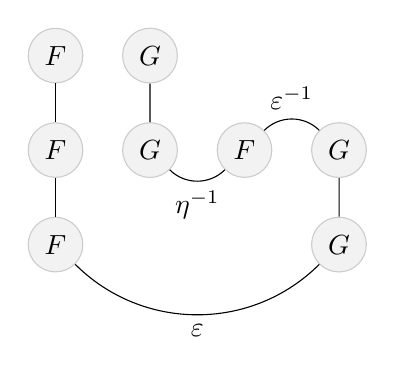
\begin{tikzpicture}[baseline=(X), scale=0.8, bend angle=45, auto, fct/.style={circle, draw=gray!40, fill=gray!10}, scale=1.5]
		\node[fct] (X0) at (0,1) {$F$};
		\node[fct] (X1) at (1,1) {$G$};

		\node[fct] (Y0) at (0,0) {$F$} edge (X0);
		\node[fct] (Y1) at (1,0) {$G$} edge (X1);
		\node[fct] (Y2) at (2,0) {$F$} edge[bend left] node {$\eta^{-1}$} (Y1);
		\node[fct] (Y3) at (3,0) {$G$} edge[bend right] node[swap] {$\varepsilon^{-1}$} (Y2);

		\node[fct] (Z0) at (0,-1) {$F$} edge (Y0);
		\node[fct] (Z1) at (3,-1) {$G$} edge (Y3) edge[bend left] node {$\varepsilon$} (Z0);
		\coordinate (X) at (0, -0.5);
	\end{tikzpicture} \quad = \quad 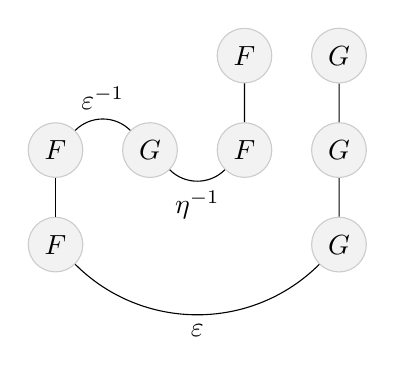
\begin{tikzpicture}[baseline=(X), scale=0.8, bend angle=45, auto, fct/.style={circle, draw=gray!40, fill=gray!10}, scale=1.5]
		\node[fct] (X0) at (2,1) {$F$};
		\node[fct] (X1) at (3,1) {$G$};
	
		\node[fct] (Y0) at (0,0) {$F$};
		\node[fct] (Y1) at (1,0) {$G$} edge[bend right] node[swap] {$\varepsilon^{-1}$} (Y0);
		\node[fct] (Y2) at (2,0) {$F$} edge[bend left] node {$\eta^{-1}$} (Y1) edge (X0);
		\node[fct] (Y3) at (3,0) {$G$} edge (X1);
	
		\node[fct] (Z0) at (0,-1) {$F$} edge (Y0);
		\node[fct] (Z1) at (3,-1) {$G$} edge (Y3) edge[bend left] node {$\varepsilon$} (Z0);
		\coordinate (X) at (0, -0.5);
	\end{tikzpicture} \end{equation}
	左边诚然是 $\varepsilon \cdot (F\eta^{-1}G) \cdot (FG\varepsilon^{-1})$ 的图解, 因为 $FG\varepsilon^{-1}$ 无非是 $\varepsilon^{-1}$ 左横合成 $\identity_F$, $\identity_G$, 依此类推. 为了过渡到右图, 将 $FG \varepsilon^{-1}: FG \to FGFG$ 表作:
	\[ \begin{tikzpicture}[baseline=(X), bend angle=70, auto, fct/.style={circle, draw=gray!40, fill=gray!10}]
		\node[fct] (X0) {$F$}; \node[fct] (X1) [right=of X0] {$G$};
		\node[fct] (Y0) [below=of X0] {$F$} edge (X0); \node[fct] (Y1) [below=of X1] {$G$} edge (X1);
		\node[fct] (Y2) [right=of Y1] {$F$};
		\node[fct] (Y3) [right=of Y2] {$G$} edge[bend right] node {$\varepsilon^{-1}$} (Y2);
		\coordinate (X) at ($(X0)!.5!(Y0)$);
	\end{tikzpicture} = \begin{tikzpicture}[baseline=(X), bend angle=70, auto, fct/.style={circle, draw=gray!40, fill=gray!10}]
		\node[fct] (X0) {$F$}; \node[fct] (X1) [right=of X0] {$G$} edge[bend left] node[swap] {$\varepsilon$} (X0);
		\node[fct] (Y0) [below=of X0] {$F$}; \node[fct] (Y1) [below=of X1] {$G$} edge[bend right] node {$\varepsilon^{-1}$} (Y0);
		\node[fct] (Y2) [right=of Y1] {$F$};
		\node[fct] (Y3) [right=of Y2] {$G$} edge[bend right] node {$\varepsilon^{-1}$} (Y2);
		\coordinate (X) at ($(X0)!.5!(Y0)$);
	\end{tikzpicture} \]
	因为与恒等函子的横合成不起作用, 上层的 $\varepsilon$ 放在左侧或右侧是一样的, 右图遂化作
	\[ \begin{tikzpicture}[baseline=(X), bend angle=70, auto, fct/.style={circle, draw=gray!40, fill=gray!10}]
		\node[fct] (X0) {$F$}; \node[fct] (X1) [right=of X0] {$G$} edge[bend left] node[swap] {$\varepsilon$} (X0);
		\node[fct] (Y0) [below=of X0] {$F$}; \node[fct] (Y1) [below=of X1] {$G$} edge[bend right] node {$\varepsilon^{-1}$} (Y0);
		\node[fct] (Y3) [left=of Y0] {$G$};
		\node[fct] (Y2) [left=of Y3] {$F$} edge[bend left] node {$\varepsilon^{-1}$} (Y3);
		\coordinate (X) at ($(X0)!.5!(Y0)$);
	\end{tikzpicture} = \begin{tikzpicture}[baseline=(X), bend angle=70, auto, fct/.style={circle, draw=gray!40, fill=gray!10}]
		\node[fct] (X0) {$F$}; \node[fct] (X1) [right=of X0] {$G$};
		\node[fct] (Y0) [below=of X0] {$F$} edge (X0); \node[fct] (Y1) [below=of X1] {$G$} edge (X1);
		\node[fct] (Y3) [left=of Y0] {$G$};
		\node[fct] (Y2) [left=of Y3] {$F$} edge[bend left] node {$\varepsilon^{-1}$} (Y3);
		\coordinate (X) at ($(X0)!.5!(Y0)$);
	\end{tikzpicture} \]
	等式右边的底部再装配 $\varepsilon \cdot (F\eta^{-1}G)$, 便是 \eqref{eqn:adj-equiv-two-expression}.

	现在来证明 \eqref{eqn:adj-zigzag-2}. 将 \eqref{eqn:adj-equiv-two-expression} 的左图代入 $\varepsilon'$, 省略函子标记以表 $(G\varepsilon')(\eta G)$ 为
	\[ 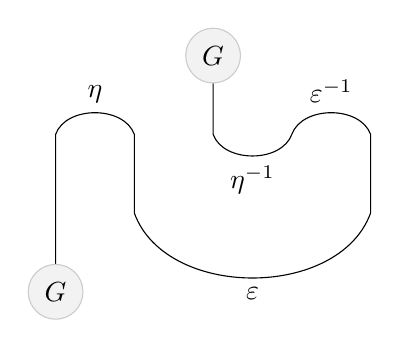
\begin{tikzpicture}[baseline=(X), bend angle=70, auto, fct/.style={circle, draw=gray!40, fill=gray!10}]
		\coordinate (A) at (0,0); \coordinate (B) at (0,2); \coordinate (C) at (1,2); \coordinate (D) at (1,1); \coordinate (E) at (4,1); \coordinate (F) at (4,2); \coordinate (G) at (3,2); \coordinate (H) at (2,2); \coordinate (I) at (2,3);
	
		\draw (A) -- (B) to[bend left] node {$\eta$} (C) -- (D) to[bend right] node[swap] {$\varepsilon$} (E) -- (F) to[bend right] node[swap] {$\varepsilon^{-1}$} (G) to[bend left] node {$\eta^{-1}$} (H) -- (I);
	
		\node[fct] at (A) {$G$}; \node[fct] at (I) {$G$};
		\coordinate (X) at (0, 1.5);
	\end{tikzpicture} \quad = \quad
	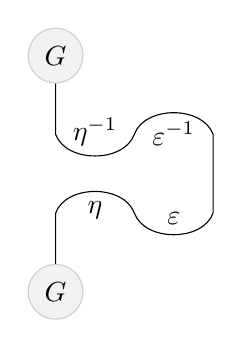
\begin{tikzpicture}[baseline=(X), bend angle=70, auto, fct/.style={circle, draw=gray!40, fill=gray!10}]
		\coordinate (A) at (0,0); \coordinate (B) at (0,1); \coordinate (C) at (1,1); \coordinate (D) at (2,1); \coordinate (E) at (2,2); \coordinate (F) at (1,2); \coordinate (G) at (0,2); \coordinate (H) at (0,3);
	
		\draw (A) -- (B) to[bend left] node[swap] {$\eta$} (C) to[bend right] node {$\varepsilon$} (D) -- (E) to[bend right] node {$\varepsilon^{-1}$} (F) to [bend left] node[swap] {$\eta^{-1}$} (G) -- (H);
		\node[fct] at (A) {$G$}; \node[fct] at (H) {$G$};
		\coordinate (X) at (0, 1.5);
	\end{tikzpicture}\]
	从左图化到右图的方法是先将图按垂直方向拉开 (即在中间插入 $\identity_F$, $\identity_G$ 等), 然后将 $\eta^{-1}$ 向左挪动, 道理和 \eqref{eqn:adj-equiv-two-expression} 的论证类似. 现在可以用 $\eta \eta^{-1} = \identity_{GF}$ 和 $\varepsilon^{-1}\varepsilon = \identity$ 来将右图化作
	\[\begin{tikzpicture}[baseline=(X), bend angle=70, auto, fct/.style={circle, draw=gray!40, fill=gray!10}]
		\node[fct] (A) {$G$}; \node[fct] (B) [above=of A] {$G$} edge (A);
		\node[fct] (C) [right=of A] {$F$}; \node[fct] (D) [above=of C] {$F$} edge (C);
		\node[fct] (E) [right=of C] {$G$} edge[bend left] node[swap] {$\varepsilon$} (C);
		\node[fct] (F) [right=of D] {$G$} edge[bend right] node {$\varepsilon^{-1}$} (D) edge (E);
		\coordinate (X) at ($(A)!.5!(B)$);
	\end{tikzpicture} \quad = \quad \begin{tikzpicture}[baseline=(X), bend angle=70, auto, fct/.style={circle, draw=gray!40, fill=gray!10}]
		\node[fct] (A) {$G$}; \node[fct] (B) [above=of A] {$G$} edge (A);
		\coordinate (X) at ($(A)!.5!(B)$);
	\end{tikzpicture}\]
	这就证出了 \eqref{eqn:adj-zigzag-2}. 至于 \eqref{eqn:adj-zigzag-1} 的情形几乎是以上论证的镜像, 唯一差别是改用  \eqref{eqn:adj-equiv-two-expression} 的右图代入 $\varepsilon'$.
	
	最后证唯一性. 假设 $\varepsilon'': FG \to \identity$ 也满足 \eqref{eqn:adj-zigzag-1} 和 \eqref{eqn:adj-zigzag-2}. 注意到 $\varepsilon''\cdot (\varepsilon' FG) = \varepsilon' \cdot (FG \varepsilon'')$; 这是因为两者对应同一个图表 $FGFG \to \identity$:
	\[\begin{tikzpicture}[baseline=(X), bend angle=45, auto, fct/.style={circle, draw=gray!40, fill=gray!10}]
		\node[fct] (F) {$F$}; \node[fct] (G) [right=of F] {$G$} edge[bend left] node[swap] {$\varepsilon'$} (F);
		\node[fct] (F1) [right=of G] {$F$}; \node[fct] (G1) [right=of F1] {$G$} edge[bend left] node[swap] {$\varepsilon''$} (F1);
		\coordinate (X) at (F);
	\end{tikzpicture}.\]
	此外易见 $(\varepsilon'F \cdot F\eta)G = \varepsilon' FG \cdot F\eta G$ 和 $F(G\varepsilon'' \cdot \eta G) = FG\varepsilon'' \cdot F\eta G$; 应用 \eqref{eqn:adj-zigzag-1} 和 \eqref{eqn:adj-zigzag-2} 可知这两者都等于 $\identity_{FG}$; 综之 $\varepsilon'' = \varepsilon'' \cdot (\varepsilon' FG) (F\eta G) = \varepsilon' (FG\varepsilon'')(F\eta G) = \varepsilon'$. 唯一性得证.
\end{proof}

范畴论中还有许多类似的可视化技巧, 读者不妨参阅 P.\ Selinger 在 \cite[Chapter 4]{Co11} 撰写的综述. 在 \S\ref{sec:braiding} 还会碰上类似的手法.

\section{极限}\label{sec:limits}
我们先给出极限的一般定义, 然后逐步剖析.

\begin{definition}\label{def:diagonal-functor}
	令 $I, \mathcal{C}$ 为范畴. 定义对角函子 $\Delta: \mathcal{C} \to \mathcal{C}^I := \text{Fct}(I, \mathcal{C})$ 如下: 它将任一 $X \in \Obj(\mathcal{C})$ 映至常值函子
	\begin{gather*}
		\Delta(X): I \longrightarrow \mathcal{C}\;
		\left\{ \begin{array}{ll}
			\forall i \in \Obj(I), & i \longmapsto X \\
			\forall [i \to j] \in \Mor(I), & [i \to j] \longmapsto [\identity_X: X \to X].
		\end{array}\right.
	\end{gather*}
	给定态射 $f: X \to Y$, 范畴 $\mathcal{C}^I$ 中 $\Delta(f): \Delta(X) \to \Delta(Y)$ 的定义是显然的: 它对每个 $i \in \Obj(I)$ 指定 $f: X \to Y$.
\end{definition}

以 $I^{\text{op}}$ 代 $I$, 同样可定义对角函子 $\Delta: \mathcal{C} \to \mathcal{C}^{I^{\text{op}}} := \text{Fct}(I^{\text{op}}, \mathcal{C})$. 回忆定义 \ref{def:comma-category} 及其后的讨论: 对于函子 $I \xrightarrow{\alpha} \mathcal{C} \xleftarrow{\beta} I^\text{op}$, 可以构造两种逗号范畴
\begin{align*}
	\left[ \mathbf{1} \xrightarrow{j_\alpha} \mathcal{C}^I \xleftarrow{\Delta} \mathcal{C} \right] & \leadsto \quad (j_\alpha/\Delta) =: (\alpha / \Delta), \\
	\left[ \mathcal{C} \xrightarrow{\Delta} \mathcal{C}^{I^\text{op}} \xleftarrow{j_\beta} \mathbf{1} \right] & \leadsto \quad (\Delta/j_\beta) =: (\Delta/\beta).
\end{align*}
\begin{definition}[极限]\label{def:limit}\index{guinajixian@归纳极限 (inductive limit)}\index{toushejixian@投射极限 (projective limit)}\index[sym1]{limind@$\varinjlim$}\index[sym1]{limproj@$\varprojlim$}
	令 $I, \mathcal{C}$ 为范畴. 考虑函子 $\alpha: I \to \mathcal{C}$ 和 $\beta: I^\text{op} \to \mathcal{C}$.
	\begin{compactenum}
		\item 逗号范畴 $(\alpha / \Delta)$ 中若存在始对象则记作 $\varinjlim \alpha$, 称为 $\alpha$ 的\emph{归纳极限};
		\item 逗号范畴 $(\Delta / \beta)$ 中若存在终对象则记作 $\varprojlim \beta$, 称为 $\beta$ 的\emph{投射极限}.
	\end{compactenum}
	我们也说它们是以 $I$ 为指标的极限.
\end{definition}
关于极限的术语尚未统一, 以下是几种常见版本.
\begin{center}\begin{tabular}{c|c}
	$\varinjlim$ & $\varprojlim$ \\
	归纳极限 & 投射极限 \\
	正向极限 & 逆向极限 \\
	余极限 ($\text{colim}$) & 极限 ($\text{lim}$)
\end{tabular}\end{center}

命题 \ref{prop:initial-obj-uniqueness} 确保各极限若存在则唯一. 更明确地说, 逗号范畴给出下述基于 $\mathcal{C}$ 中交换图表的描述
\begin{equation*}\begin{gathered}
	(\alpha/\Delta): \left\{ \begin{array}{ll}
		\text{对象}: & \left( L, (\alpha(i) \xrightarrow{f_i} L)_{i \in \Obj(I)} \right), \quad \forall\; [i \xrightarrow{\phi} j], \;
			\begin{tikzcd}[column sep=tiny, row sep=tiny]
				\alpha(i) \arrow[rd] \arrow[rr, "{\alpha(\phi)}"] & & \alpha(j) \arrow[ld] \\
				{} & L &
			\end{tikzcd} \\
		\text{态射}: & \left[ \varphi: (L, (f_i)_i) \to (L', (f'_i)_i) \right] =  \forall i, \;
			\begin{tikzcd}[column sep=tiny, row sep=small]
				\alpha(i) \arrow[r, "f_i"] \arrow[rd, "f'_i"'] & L \arrow[d, "\varphi"] \\
				{} & L'
			\end{tikzcd}
	\end{array}\right. \\
	(\Delta/\beta): \left\{ \begin{array}{ll}
		\text{对象}: & \left( L, (L \xrightarrow{g_i} \beta(i))_{i \in \Obj(I)} \right), \quad \forall\; [i \xrightarrow{\phi} j], \;
			\begin{tikzcd}[column sep=tiny, row sep=tiny]
				\beta(i) & & \beta(j) \arrow[ll, "\beta(\phi)"'] \\
				{} & L \arrow[lu] \arrow[ru] &
			\end{tikzcd} \\
		\text{态射}: & \left[ \varphi: (L, (g_i)_i) \to (L', (g'_i)_i) \right] =  \forall i, \;
			\begin{tikzcd}[column sep=tiny, row sep=small]
				\beta(i) & L \arrow[d, "\varphi"] \arrow[l, "g_i"'] \\
				{} & L' \arrow[lu, "g'_i"]
			\end{tikzcd}
	\end{array}\right.
\end{gathered}\end{equation*}

一些文献将 $(\alpha/\Delta)$ 和 $(\Delta/\beta)$ 的对象分别称作锥和余锥, 这是直观的.

依此, $\alpha$ 的归纳极限可以重新理解为资料 $(\varinjlim \alpha, \alpha(i) \xrightarrow{\iota_i} \varinjlim \alpha)$, 而 $\beta$ 的投射极限为资料 $(\varprojlim \beta, p_i: \varprojlim \beta \xrightarrow{p_i} \beta(i))$, 各自的泛性质图解为
\begin{equation}\label{eqn:lim-diagrams}\begin{tikzcd}
	\alpha(i) \arrow[rd, "{\iota_i}"] \arrow[rdd] \arrow[rr, "{\alpha(\phi)}"] & & \alpha(j) \arrow[ld, "{\iota_j}"'] \arrow[ldd] \\
	& \varinjlim \alpha \arrow[dashed, d, "\exists !"] &  \\
	& L &
	\end{tikzcd}\quad\begin{tikzcd}
	\beta(i) & & \beta(j) \arrow[ll, "{\beta(\phi)}"'] \\
	& \varprojlim \beta \arrow[lu, "p_i"'] \arrow[ru, "p_j"] & \\
	& L \arrow[luu] \arrow[ruu] \arrow[dashed, u, "{\exists !}"'] &
\end{tikzcd}\end{equation}
图表的读法是: 对每个 $(\alpha / \Delta)$ 或 $(\Delta/\beta)$ 的对象 $(L, \ldots)$, 图中存在唯一的态射 $\dashrightarrow$ 使得全图对任意 $\phi \in \Mor(I)$ 皆交换.

\begin{remark}\label{rem:lim-duality}
	注意到 \eqref{eqn:lim-diagrams} 中两图箭头反向. 其实 $\varinjlim$ 和 $\varprojlim$ 是对偶的概念: 设 $\alpha: I \to \mathcal{C}$, 对反范畴有相应的 $\alpha^\text{op}: I^\text{op} \to \mathcal{C}^\text{op}$ (注记 \ref{rem:op-functor}). 对 $I^\text{op}$ 和 $\mathcal{C}^\text{op}$ 仍有相应的对角函子 $\Delta^{\text{op}}$. 从而导出
	\begin{align*}
		(\alpha / \Delta)^\text{op} & = (\Delta^\text{op} / \alpha^\text{op}), \\
		\varprojlim (\alpha^{\text{op}}) & = \varinjlim \alpha, \quad \text{假设任一侧的极限存在}.
	\end{align*}
\end{remark}

\begin{lemma}\label{prop:lim-functoriality}
	设 $\psi: \alpha \to \alpha'$ 是函子范畴 $\mathcal{C}^I$ 中的态射, 假定相应的 $\varinjlim$ 皆存在, 则存在唯一的态射 $\varinjlim \psi$ 使得
	\begin{tikzcd}[row sep=small, column sep=small]
		\alpha(i) \arrow[r] \arrow[d, "\psi(i)"'] & \varinjlim \alpha \arrow[d, "\varinjlim\psi"] \\
		\alpha'(i) \arrow[r] & \varinjlim \alpha'
	\end{tikzcd}
	对每个 $i$ 皆交换. 若 $\alpha \xrightarrow{\psi_1} \alpha' \xrightarrow{\psi_2} \alpha''$, 则 $\varinjlim (\psi_2 \psi_1) = \varinjlim \psi_2 \varinjlim \psi_1$. 对 $\varprojlim$ 也有类似的结果: $\psi: \beta \to \beta'$ 自然地诱导出 $\varprojlim \beta \to \varprojlim \beta'$ 等等.
\end{lemma}
\begin{proof}
	在 $\varinjlim \alpha$ 的泛性质中考虑 $L := \varinjlim \alpha' \leftarrow \alpha'(i) \xleftarrow{\psi(i)} \alpha(i)$ 即可. 性质 $\varinjlim (\psi_2 \psi_1) = \varinjlim \psi_2 \varinjlim \psi_1$ 源自
	\[\begin{tikzcd}[row sep=small, column sep=small]
		\alpha(i) \arrow[r] \arrow[d] & \alpha'(i) \arrow[r] \arrow[d] & \alpha''(i) \arrow[d] \\
		\varinjlim \alpha \arrow[r] & \varinjlim \alpha' \arrow[r] & \varinjlim \alpha''
	\end{tikzcd} \qquad i \in \Obj(I) \]
	全图的交换性.
\end{proof}

以下遵循约定 \ref{con:U-small}, 区分范畴与小范畴. 我们仅考虑 $I$ 是小范畴情形的极限. 这主要是为了陈述方便, 而且按假设 \ref{hyp:universe} 总能扩大所选的宇宙 $\mathcal{U}$ 使得所论的范畴都是小范畴. 但也请读者先留个心眼, 因为在一些场合下集合的大小确实会造成实质差异, 例如下面要提到的命题 \ref{prop:preorder-complete}.

\begin{example}\label{eg:set-limits}
	取 $\mathcal{C} := \cate{Set}$ 并设 $I$ 是小范畴. 我们先构造 $\varprojlim \beta$. 定义
	\begin{align*}
		\varprojlim \beta & := \left\{ (x_i)_{i \in \Obj(I)} \in \prod_i \beta(i) : \forall \sigma \in \Hom_I(i,j), \; \beta(\sigma)(x_j) = x_i \right\} \\
		& = \Ker\left[ \prod_i \beta(i) \rightrightarrows \prod_\sigma \beta(s(\sigma)) \right] \quad \text{(等化子)},
	\end{align*}
	$\Ker[\cdots]$ 的双箭头分别以映射 $(x_i)_i \mapsto x_{s(\sigma)}$ 和 $(x_i)_i \mapsto \beta(\sigma)\left(x_{t(\sigma)}\right)$ 为其``$\sigma$-坐标'', 其中 $\sigma$ 取遍 $I$ 中态射. 上式是 $\cate{Set}$ 的一个对象, 它带有一族投影映射 $p_j: \varprojlim \beta \to \beta(j)$, $p_j((x_i)_i) = x_j$, 其中 $j$ 取遍 $\Obj(I)$. 不难验证 $(\varprojlim \beta, (p_j)_j)$ 是 $\beta$ 的投射极限.

	接着考虑 $\alpha: I \to \cate{Set}$. 定义
	\[ \varinjlim \alpha := \left( \bigsqcup_{i \in \Obj(I)} \alpha(i) \right) \Big/ \sim \]
	其中 $\bigsqcup_i \alpha(i)$ 代表无交并, $\sim$ 是下述关系生成的等价关系
	\[ x \sim \alpha(\sigma)(x), \quad \sigma: i \to j, \quad x \in \alpha(i). \]
	由商集的性质得到一族映射 $\iota_j: \alpha(j) \to \varinjlim \alpha$, 其中 $j$ 取遍 $\Obj(I)$; 它映 $x \in \alpha(j)$ 至含 $x$ 的等价类. 不难验证 $(\varinjlim \alpha, (\iota_j)_j)$ 是 $\alpha$ 的归纳极限.
\end{example}
上述构造有一个明显缺陷: 它仅说明如何``生成''等价关系 $\sim$, 却没有直接的描述. 弥补这点需要对 $I$ 施加进一步的条件, 我们顺势引入滤过范畴的概念.

\begin{definition}\label{def:filtrant-cat}\index{luguofanchou@滤过范畴 (filtered category)}
	非空范畴 $I$ 若满足以下条件, 则称为\emph{滤过}的:
	\begin{compactitem}
		\item 对任意 $i, j \in \Obj(I)$ 存在 $k \in \Obj(I)$ 及态射 $i \to k$, $j \to k$;
		\item 对任意箭头 $f,g: i \to j$, 存在 $k \in \Obj(I)$ 和 $h: j \to k$, 使得 $hf = hg$.
	\end{compactitem}
\end{definition}
对于来自非空偏序集 $(I, \leq)$ 的范畴, 第二个条件是多余的, 此时我们回到 \S\ref{sec:group-limit} 定义之滤过偏序概念. 例如偏序集 $(\Z_{\geq 1}, \leq)$ 便是滤过偏序集.

现在回到例 \ref{eg:set-limits} 的函子 $\alpha: I \to \cate{Set}$ 并假设 $I$ 滤过. 在无交并 $\bigsqcup_{i \in \Obj(I)} \alpha(i)$ 上定义关系 $\sim$ 如下: 对任意 $i, j \in \Obj(I)$ 及 $x_i \in \alpha(i)$, $x_j \in \alpha(j)$, 若
\begin{equation}\label{eqn:filtrant-equiv} \text{存在} \begin{cases}
	f: i \to k, \\
	g: j \to k
	\end{cases}
	\text{使得} \quad \alpha(f)(x_i) = \alpha(g)(x_j) \in \alpha(k)
\end{equation}
则定 $x_i \sim x_j$, 显然例 \ref{eg:set-limits} 中的等价关系也必须满足这个性质, 若我们能说明 $\sim$ 已然是等价关系, 则这里的 $\sim$ 就是例 \ref{eg:set-limits} 中的 $\sim$. 反身性和对称性实属显然, 现验证传递性如下: 设 $(x_i \sim x_j) \wedge (x_j \sim x_k)$, 存在图表
\[ \begin{tikzcd}[scale=0.75]
	i \arrow[rd] & & j \arrow[ld] \arrow[rd] & & k \arrow[ld] \\
	& h \arrow[dashed, rd] & & h' \arrow[dashed, ld] & \\
	& & g & &
\end{tikzcd} \quad \begin{tikzcd}[scale=0.75]
	x_i \arrow[mapsto, rd] & & x_j \arrow[mapsto, ld] \arrow[mapsto, rd] & & x_k \arrow[mapsto, ld] \\
	& x_h \arrow[dashed, rd] & & x_{h'} \arrow[dashed, mapsto, ld] & \\
	& & ? & & 
\end{tikzcd} \]
其中的虚线箭头和 $g$ 由定义 \ref{def:filtrant-cat} 的第一条补全. 然而 $x_h$ 和 $x_{h'}$ 在虚箭头下的像未必相同, 为此我们利用定义第二条找到 $I$ 中态射 $g \to g'$, 使得合成态射 $j \to h \to g \to g'$ 同 $j \to h' \to g \to g'$ 相等; 在图表中以 $g'$ 代 $g$ 便可确保 $x_i \sim x_k$. 故 $\sim$ 为等价关系. 由 $\sim$ 的定义亦可导出 \eqref{eqn:lim-diagrams} 的左图交换. 综之,
\[ \varinjlim \alpha := \bigsqcup_{i \in \Obj(I)} \alpha(i) \big/ \sim \]
尔后我们还会在不同范畴中反复考虑滤过的 $\varinjlim$.

\begin{example}\label{eg:top-limits}
	同样方法可构造范畴 $\mathcal{C} := \cate{Top}$ 中的极限. 对于小范畴 $I$, 极限 $(\varinjlim \alpha, \iota_j)$ 和 $(\varprojlim \beta, p_j)$ 的构造与 $\cate{Set}$ 完全相同, 只消赋予这些集合商拓扑或子空间拓扑 \cite[\S 3.1, \S 3.4]{Xiong}.
\end{example}

给定范畴 $\mathcal{C}$. 尽管所论的极限在 $\mathcal{C}$ 中未必存在, 一旦将 $\mathcal{C}$ 嵌入函子范畴 $\mathcal{C}^\wedge$ 或 $\mathcal{C}^\vee$ (参考 \S\ref{sec:representable-functors}), 则能确保所有(小)极限的存在性.

\begin{proposition}\label{prop:lim-Yoneda}
	设 $I$ 为小范畴, 函子 $\alpha: I \to \mathcal{C}^\wedge$ 的极限由如下定义的对象 $\Yinjlim \alpha \in \Obj(\mathcal{C}^\wedge)$
	\begin{gather*}
		\Yinjlim \alpha: S \longmapsto \varinjlim \left( \alpha(S) \right), \\
		[T \xrightarrow{f} S] \leadsto \varinjlim \alpha(S) \xrightarrow{\varinjlim \alpha(f)} \varinjlim \alpha(T),
	\end{gather*}
	连同自然态射族 $\alpha(j)(\cdot) \to \varinjlim \alpha(\cdot)$ 给出, 其中 $j \in \Obj(I)$ 而 $\varinjlim \alpha(f)$ 的构造见引理 \ref{prop:lim-functoriality}; 这里不带引号的 $\varinjlim$ 是 $\cate{Set}$ 中的极限. 类似地, 函子 $\beta: I^\text{op} \to \mathcal{C}^\wedge$ 的极限由
	\[ \Yprojlim \beta: S \longmapsto \varprojlim \left( \beta(S) \right) \]
	等资料给出. 类似性质对取值在 $\mathcal{C}^\vee$ 的情形同样成立, 我们在符号上将这些极限不予区分地记作
	\begin{align*}
		\Yinjlim \alpha: S & \longmapsto \varinjlim \left( \alpha(S) \right), \quad \alpha: I \to \mathcal{C}^\wedge \;\text{或}\; \mathcal{C}^\vee, \\
		\Yprojlim \beta: S & \longmapsto \varprojlim \left( \beta(S) \right), \quad \beta: I^\text{op} \to \mathcal{C}^\wedge \;\text{或}\; \mathcal{C}^\vee.
	\end{align*}
\end{proposition}
\begin{proof}
	诀窍是对函子逐点地 (或逐对象地) 取极限以化约到 $\cate{Set}$ 情形, 仅以 $\alpha: I \to \mathcal{C}^\wedge$ 和 $\Yinjlim \alpha$ 的情形阐释. 考虑相应的图表 \eqref{eqn:lim-diagrams} 并给定 $L \in \mathcal{C}^\wedge$ 和一族态射 $\alpha(i) \to L$. 对于每个 $S \in \Obj(\mathcal{C})$, 根据 $\cate{Set}$ 中 $\varinjlim$ 的构造可知存在唯一的 $\varphi(S)$ 使得图表
	\begin{tikzcd}[column sep=tiny, row sep=tiny]
		\alpha(i)(S) \arrow[rr] \arrow[rd] & & \varinjlim \alpha(S) \arrow[ld, "\varphi(S)"] \\
		& L(S) &
	\end{tikzcd}
	对所有 $i$ 交换. 关键在于证明这些 $\varphi(\cdot)$ 能在 $\mathcal{C}^\wedge$ 中拼为 $\Yinjlim \alpha \xrightarrow{\varphi} L$. 考虑 $\mathcal{C}$ 中任意态射 $f: T \to S$, 以下将 $L(S)$ 视同常值函子 $\Delta(L(S)): I \to \cate{Set}$, 易见其 $\varinjlim$ 是 $L(S)$ 自身 (请验证); 对 $L(T)$ 亦同. 于是由引理 \ref{prop:lim-functoriality} 导出: 对每个 $i \in \Obj(I)$
	\[ \begin{tikzcd}
		\alpha(i)(S) \arrow[r, "\alpha(i)(f)"] \arrow[d] & \alpha(i)(T) \arrow[d] \\
		L(S) \arrow[r, "L(f)"'] & L(T)
	\end{tikzcd} \;\text{交换, 故} \;
	\begin{tikzcd}
		\varinjlim \alpha(S) \arrow[r, "{\varinjlim \alpha(f)}", yshift=0.5em] \arrow[d, "\varphi(S)"'] & \varinjlim \alpha(T) \arrow[d, "\varphi(T)"] \\
		L(S) \arrow[r, "L(f)"'] & L(T)
	\end{tikzcd} \;\text{交换}, \]
	而右图就是 $\varphi(\cdot)$ 所需的函子性.
\end{proof}
如此一来, 极限的存在性就归结为函子的可表性, 见 \S\ref{sec:representable-functors}.

\begin{proposition}\label{prop:lim-as-fct}
	设 $I$ 为小范畴. 以下我们利用函子 $k_{\mathcal{C}}$ 和 $h_{\mathcal{C}}$, 分别将 $\mathcal{C}$ 看作 $\mathcal{C}^\vee$ 和 $\mathcal{C}^\wedge$ 的子范畴.
	\begin{enumerate}
		\item 函子 $\alpha: I \to \mathcal{C}$ 的归纳极限存在当且仅当 $\Yinjlim \alpha \in \mathcal{C}^\vee$ 可表; 给定 $\alpha$ 的极限相当于给定对象 $\varinjlim \alpha \in \Obj(\mathcal{C})$ 连同一个同构 $k_{\mathcal{C}}(\varinjlim \alpha) \rightiso \Yinjlim \alpha$.
		\item 函子 $\beta: I^\text{op} \to \mathcal{C}$ 的投射极限存在当且仅当 $\Yprojlim \beta \in \mathcal{C}^\wedge$ 可表; 给定 $\beta$ 的极限相当于给定对象 $\varprojlim \beta \in \Obj(\mathcal{C})$ 连同一个同构 $h_{\mathcal{C}}(\varprojlim \beta) \rightiso \Yprojlim \beta$.
	\end{enumerate}
\end{proposition}
极限的性质遂可简洁地刻画为
\begin{align*}
	\Hom_{\mathcal{C}}(\varinjlim \alpha, \cdot) & \rightiso \varprojlim_i \Hom_{\mathcal{C}}(\alpha(i), \cdot) = \Yinjlim \alpha, \\
	\Hom_{\mathcal{C}}(\cdot, \varprojlim \beta) & \rightiso \varprojlim_i \Hom_{\mathcal{C}}(\cdot, \beta(i)) = \Yprojlim \beta.
\end{align*}
注意到这里的 $\mathcal{C}^\vee$ 与 $\mathcal{C}^\wedge$ 不能互换: 在 $\Hom_{\mathcal{C}}$ 外头的极限必须是 $\varprojlim$!

\begin{proof}
	先考虑归纳极限的情形. 将 \eqref{eqn:lim-diagrams} 中的泛性质改写为: 给定 $\alpha$ 的极限相当于给定对象 $\varinjlim \alpha \in \Obj(\mathcal{C})$, 连同一族态射 $\iota_i: \alpha(i) \to \varinjlim \alpha$, 使得函子间的态射
	\begin{equation*}\begin{tikzcd}[row sep=small]
		k_{\mathcal{C}}(\varinjlim \alpha) \arrow[equal, r] & \Hom_{\mathcal{C}}(\varinjlim \alpha , \cdot) \arrow[r, "\xi"] & \varprojlim_i \Hom_{\mathcal{C}}(\alpha(i), \cdot) & \Yinjlim \alpha \arrow[equal, l] \\
		& f \arrow[phantom, u, sloped, "\in" description] \arrow[mapsto, r] & (\iota_i^* f = f \circ \iota_i)_{i \in \Obj(I)} \arrow[phantom, u, sloped, "\in" description] &
	\end{tikzcd}\end{equation*}
	为同构. 反过来说, 任何同构 $\xi: k_{\mathcal{C}}(\varinjlim \alpha) \rightiso \Yinjlim \alpha$ 都可由一族 $\iota_i: \alpha(i) \to \varinjlim \alpha$ 如是导出: 这是定理 \ref{prop:Yoneda-lemma} 的应用, 或者更直截了当地将上图的变元取为 $\varinjlim \alpha$, 则 $f = \identity$ 的像就是所求的 $(\iota_i)_i$.

	投射极限的处理方法完全类似, 此时考察的同构是
	\begin{equation*}\begin{tikzcd}[row sep=small]
		\Hom_{\mathcal{C}}(\cdot, \varprojlim \beta) \arrow[r] & \varprojlim_i \Hom_{\mathcal{C}}(\cdot, \beta(i)) = \Yprojlim \beta \\
		f \arrow[phantom, u, sloped, "\in" description] \arrow[mapsto, r] & (p_{i *} f = p_i \circ f)_{i \in \Obj(I)} \arrow[phantom, u, sloped, "\in" description]
	\end{tikzcd}\end{equation*}
	明所欲证.
\end{proof}

命题 \ref{prop:lim-as-fct} 可将极限的许多性质化约到集合情形, 实质地简化论证. 我们且看一个例子.
\begin{lemma}\label{prop:lim-Fubini}
	设 $I, J$ 为小范畴, 假设 $\mathcal{C}$ 中具有以 $I$, $J$ 为指标的 $\varinjlim$. 考虑函子 $\alpha: I \times J \to \mathcal{C}$, 存在典范同构
	\[ \varinjlim_j \left( \varinjlim\alpha(\cdot, j) \right) \simeq \varinjlim \alpha \simeq \varinjlim_i \left( \varinjlim\alpha(i, \cdot) \right) \]
	其中左项极限先对 $I$ 再对 $J$ 取, 右项反之. 投射极限 $\varprojlim \beta$ 的情形类似.
\end{lemma}
\begin{proof}
	证 $\varinjlim$ 情形即足. 给定 $I$ 中的态射 $i \to i'$, 引理 \ref{prop:lim-functoriality} 对每个 $j$ 给出自然的交换图表
	\[ \begin{tikzcd}
		\varinjlim \alpha(i, \cdot) \arrow[r] & \varinjlim \alpha(i', \cdot) \\
		\alpha(i, j) \arrow[r] \arrow[u] & \alpha(i', j) \arrow[u]
	\end{tikzcd} \]
	因此断言中左项的极限有意义, 右项亦同. 命题 \ref{prop:lim-as-fct} 将断言化约到范畴 $\mathcal{C} = \cate{Set}$ 中的 $\varprojlim$ 情形, 后者从例 \ref{eg:set-limits} 的构造看乃是自明的.
\end{proof}

如果范畴 $I$ 的对象和态射集皆为有限集, 相应的极限称为有限极限, 此时常用图表来描述 $I$ 的构造. 极限可以分成两步来构造: 积 (或余积) 与等化子 (或余等化子); 以下讨论中都假设所论极限存在.
\begin{asparaenum}\index{yuji@余积 (coproduct)}\index{ji@积 (product)}
	\item 取 $I$ 为离散范畴, 不妨把 $I$ 等同于 $\Obj(I)$. 此时 $\varinjlim \alpha(i)$ 称作对象 $X_i := \alpha(i)$ 的\emph{余积}, 写作 $\coprod_{i \in I} X_i$; 相应地, $\prod_{i \in I} Y_i := \varprojlim \beta(i)$ 称作对象 $Y_i := \beta(i)$ 的\emph{积}. 泛性质 \eqref{eqn:lim-diagrams} 化作
		\[\begin{tikzcd}[row sep=small, column sep=small]
			\Hom_{\mathcal{C}} \left( \displaystyle\coprod_{i \in I} X_i, \cdot \right) \arrow[r, "\sim"] & \displaystyle\prod_{i \in I} \Hom_{\mathcal{C}}(X_i, \cdot) & \Hom_{\mathcal{C}} \left( \cdot, \displaystyle\prod_{i \in I} Y_i \right)  \arrow[r, "\sim"] & \displaystyle\prod_{i \in I} \Hom_{\mathcal{C}}(\cdot, Y_i) \\
			\phi \arrow[mapsto, r] & (\phi \iota_i)_{i \in I} & \phi \arrow[mapsto, r] & (p_i \phi)_{i \in I}
		\end{tikzcd}\]
		此处用到态射 $\iota_j: X_j \to \coprod_i X_i$ 和 $p_j: \prod_i Y_i \to Y_j$, 后者称为到 $Y_j$ 的投影.

		有限个对象的余积或积习惯写作 $X_1 \sqcup \cdots \sqcup X_n$ 或 $Y_1 \times \cdots \times Y_n$. 这些符号兼容于 $\cate{Set}$ 与 $\cate{Top}$ 情形下的惯例 (积空间, 无交并).
	\item 取空范畴 $I = \mathbf{0}$, 此时 \eqref{eqn:lim-diagrams} 表明 $\varinjlim$ 是始对象而 $\varprojlim$ 是终对象. 它们也可以分别被理解为空余积和空积.
	\item 取 $I$ 为图表
		\begin{tikzcd}
			\bullet \arrow[r, yshift=0.5ex] \arrow[r, yshift=-0.5ex] & \bullet
		\end{tikzcd}
		给出的范畴 (两个对象, 两个非 $\identity$ 的态射), 显然 $I^\text{op} \simeq I$. 函子 $\alpha: I \to \mathcal{C}$ 或 $\beta: I^\text{op} \to \mathcal{C}$ 可以理解为 $\mathcal{C}$ 中两个平行箭头
		\begin{tikzcd}
			X \arrow[yshift=0.5ex, r, "f"] \arrow[yshift=-0.5ex, r, "g"'] & Y ;
		\end{tikzcd}
		相应的极限记为 $\Coker(f,g) := \varinjlim \alpha$ (称为\emph{余等化子}), $\Ker(f,g) := \varprojlim \beta$ (称为\emph{等化子} 或差核). 等化子 $\Ker(f,g)$ 的泛性质表作 \index{yudenghuazi@余等化子 (coequalizer)}\index{denghuazi@等化子 (equalizer)}\index[sym1]{Ker@$\Ker$}\index[sym1]{Coker@$\Coker$}
		\begin{equation}\label{eqn:equalizer}\begin{tikzcd}
			{} & L \arrow[dashed, ld, "\exists !"'] \arrow[d, "\phi"] \arrow[rd] & \\
			\Ker(f,g) \arrow[r] & X \arrow[yshift=0.5ex, r, "f"] \arrow[yshift=-0.5ex, r, "g"'] & Y
		\end{tikzcd}\end{equation}
		意谓: 两合成态射 $\Ker(f,g) \to X \xrightarrow{f} Y$ 和 $\Ker(f,g) \to X \xrightarrow{g} Y$ 相等, 而且对任意 $\phi: L \to X$, 若 $f\phi = g\phi$ 则存在唯一的态射 $L \dasharrow \Ker(f,g)$ 使左三角交换. 同理, 余等化子的泛性质表作
		\begin{equation}\label{eqn:coequalizer}\begin{tikzcd}
			{} & L & \\
			X \arrow[yshift=0.5ex, r, "f"] \arrow[yshift=-0.5ex, r, "g"'] \arrow[ru] & Y \arrow[r] \arrow[u, "\psi"] & \Coker(f,g) \arrow[dashed, lu, "\exists !"'],
		\end{tikzcd}\end{equation}
		意谓: $X \xrightarrow{f} Y \to \Coker(f,g)$ 等于 $X \xrightarrow{g} Y \to \Coker(f,g)$, 而且对任意 $\psi: Y \to L$, 若 $\psi f = \psi g$ 则存在唯一的 $\Coker(f,g) \dasharrow L$ 使右三角交换.

		当 $\mathcal{C} = \cate{Set}$ 时, $f, g: X \rightrightarrows Y$ 的等化子是子集 $\{x: f(x)=g(x)\} \hookrightarrow X$, 余等化子是商集 $Y \twoheadrightarrow Y/\sim$, 其中 $\sim$ 是由 $f(x) \sim g(x)$ 生成的等价关系; $\mathcal{C} = \cate{Top}$ 的情况类似.
\end{asparaenum}
研究一般极限的性质前, 先对以上特例搜集一些简单的性质.

\begin{lemma}[积和余积的结合约束]\label{prop:product-associativity}\index{jieheyueshu@结合约束 (associativity constraint)}
	设有小集合的无交并分解 $I = \bigsqcup_{j \in J}  I_j$. 若范畴 $\mathcal{C}$ 具有以 $J$ 和每个 $I_j$ 为指标的积, 则以 $I$ 为指标的积也存在. 而且有唯一的同构 $a$ 及交换图表如下
	\[\begin{tikzcd}[row sep=small]
		 \prod_{i \in I} X_i \arrow[rr, "a", "\sim"'] \arrow[rd, "p_k"'] & & \prod_{j \in J} \left( \prod_{i \in I_j} X_i \right) \arrow[ld, "p_k p_j"] \\
		 & X_k & 
	\end{tikzcd} \qquad j \in J, \; k \in I_j. \]
	同样断言对余积和态射 $\iota_k: X_k \to \coprod_{i \in I} X_i$ 等也成立.
\end{lemma}
以上结果称为``结合约束''而非结合律, 因为它体现为一个唯一的同构而非等号. 以下结果表明积和余积也具有某种``交换约束''. 其证明皆可仿照引理 \ref{prop:lim-Fubini} 的论证, 化归为熟知的集合情形.
\begin{lemma}[积和余积的交换约束]\label{prop:product-commutativity}\index{jiaohuanyueshu@交换约束 (commutativity constraint)}
	设 $\sigma: I \to I$ 为小集合的双射. 设范畴 $\mathcal{C}$ 具有以 $I$ 为指标的积, $\{X_i\}_{i \in I}$ 为一族对象, 则有唯一的同构 $c$ 及交换图表如下
	\[\begin{tikzcd}[row sep=small]
		\prod_{i \in I} X_i \arrow[rr, "c", "\sim"'] \arrow[rd, "p_j"'] & & \prod_{i \in I} X_{\sigma(i)} \arrow[ld, "p_{\sigma^{-1}(j)}"] \\
		& X_j &
	\end{tikzcd} \qquad j \in I. \]
	同样断言对余积和态射 $\iota_j: X_j \to \coprod_{i \in I} X_i$ 等也成立.
\end{lemma}

\begin{lemma}
	设 $f,g: X \to Y$. 若 $\Ker(f,g)$ 存在则 $\Ker(f,g) \to X$ 是单态射. 若 $\Coker(f,g)$ 存在则 $Y \to \Coker(f,g)$ 是满态射.
\end{lemma}
\begin{proof}
	若态射 $\mu, \nu: L \rightrightarrows \Ker(f,g)$ 与 $\Ker(f,g) \to X$ 的合成是同一个态射 $\phi: L \to X$, 那么 $f\phi = g\phi$, 则在交换图表 \eqref{eqn:equalizer} 中可将 $\dasharrow$ 取为 $\mu$ 或 $\nu$, 从唯一性得知 $\mu=\nu$. 故 $\Ker(f,g) \to X$ 是单的. 倒转箭头可证 $\Coker(f,g)$ 的情形.
\end{proof}

\section{完备性}
极限能够统摄数学实践中许多重要的构造, 如拓扑学中的积空间, 商空间等. 在为数学问题制定范畴时, 我们自然也希望其中具有充分多的极限. 这就引向了以下概念.

\begin{definition}\label{def:completeness}\index{fanchou!完备 (complete)}\index{fanchou!余完备 (co-complete)}
	对于范畴 $\mathcal{C}$, 若对有所有小范畴 $I$, 所有以 $I$ 为指标的 $\varprojlim$ 都存在, 则称之为\emph{完备}的; 若所有以 $I$ 为指标的 $\varinjlim$ 都存在, 则称之为\emph{余完备}的.
\end{definition}
举例明之, $\cate{Set}$ 既是完备也是余完备的, 见例 \ref{eg:set-limits}. 定义中如不要求 $\mathcal{C}$ 比 $I$ 来得``大'', 应用范围将大大地受限. 请看以下结果.
\begin{proposition}[P.\ Freyd]\label{prop:preorder-complete}
	小范畴 $\mathcal{C}$ 完备当且仅当 $\mathcal{C}$ 来自一个预序集 $(P, \leq)$ (例 \ref{eg:categories}), 其中每个子集都有下确界.
\end{proposition}
\begin{proof}
	假设 $\mathcal{C}$ 完备. 假若存在相异的态射 $f, g: X \to Y$, 对于小集合 $I$ 可构造 $\prod_{i \in I} Y$, 故 $\Hom_{\mathcal{C}}(X, \prod_{i \in I} Y) \supset \{f, g\}^I$. 取 $|I| = |\Mor(\mathcal{C})|$ 并运用定理 \ref{prop:Cantor} 便导出矛盾. 因此 $\mathcal{C}$ 是预序集. 另一方面, 从 \eqref{eqn:lim-diagrams} 不难看出一个预序集 $(P, \leq)$ 中的 $\varprojlim \beta$ 无非是子集 $\{\beta(i) : i \in \Obj(I) \}$ 的下确界; 注意到下确界在同构意义下是唯一的. 证毕.
\end{proof}

\begin{theorem}\label{prop:limit-buildingblocks}
	设 $I$ 为小范畴, $\mathcal{C}$ 为范畴.
	\begin{compactenum}
		\item 若对所有子集 $J \subset \Mor(I)$ 和 $\mathcal{C}$ 中的对象族 $(X_j)_{j \in J}$ 都存在 $\prod_{j \in J} X_j$, 而且对所有 $f, g: X \to Y$ 都存在 $\Ker(f,g)$, 则 $\mathcal{C}$ 有所有以 $I$ 为指标的 $\varprojlim$.
		\item 若对所有子集 $J \subset \Mor(I)$ 和 $(X_j)_{j \in J}$ 都存在 $\coprod_{j \in J} X_j$, 而且对所有 $f, g: X \to Y$ 都存在 $\Coker(f,g)$, 则 $\mathcal{C}$ 有所有以 $I$ 为指标的 $\varinjlim$.
	\end{compactenum}
\end{theorem}
\begin{proof}
	两断言显然对偶, 以 $\mathcal{C}^\text{op}$ 代 $\mathcal{C}$ 可互相过渡. 故以下仅考虑 $\varprojlim$ 情形.

	考虑函子 $\beta: I^\text{op} \to \mathcal{C}$. 对于 $I$ 中的态射 $\sigma: i \to j$, 请回忆早先定义的来源 $s(\sigma)=i$ 与目标 $t(\sigma)=j$. 构造积 $\prod_{i \in \Obj(I)} \beta(i)$ 与 $\prod_{\sigma \in \Mor(I)} \beta(s(\sigma))$. 对每个 $\sigma \in \Mor(I)$ 定义一对态射
	\[\begin{tikzcd}[row sep=tiny]
		\prod_{i \in \Obj(I)} \beta(i) \arrow[bend left=15, rr, "{p_{s(\sigma)}}"] \arrow[bend right=15, rd, "{p_{t(\sigma)}}"'] & & \beta(s(\sigma)) \\
		& \beta(t(\sigma)) \arrow[ru, bend right=15, "{\beta(\sigma)}"'] &
	\end{tikzcd}\]
	故从积的泛性质导出相应的态射
	\begin{tikzcd}
		\displaystyle\prod_{i \in \Obj(I)} \beta(i) \arrow[yshift=0.5ex, r, "f"] \arrow[yshift=-0.5ex, r, "g"'] & \displaystyle\prod_{\sigma \in \Mor(I)} \beta(s(\sigma))
	\end{tikzcd}.
	今断言下述资料构成了所欲的 $\varprojlim\beta$:
	\begin{equation}\label{eqn:lim-as-ker}
		\Ker(f,g), \quad \left(q_j: \Ker(f,g) \to \prod_{i \in \Obj(I)} \beta(i) \xrightarrow{p_j} \beta(j) \right)_{j \in \Obj(I)}.
	\end{equation}

	根据例 \ref{eg:set-limits} 中的极限构造和命题 \ref{prop:lim-Yoneda} 在 $\mathcal{C}^\wedge$ 中操作, 知函子 $\Yprojlim \beta$ 等于
	\begin{align*}
		\varprojlim_i \Hom_{\mathcal{C}}(\cdot, \beta(i)) & = \Ker\left[ \prod_i \Hom_{\mathcal{C}}(\cdot, \beta(i)) \rightrightarrows \prod_\sigma \Hom_{\mathcal{C}}(\cdot, \beta(s(\sigma)))  \right] \\
		& = \Hom_{\mathcal{C}}\left( \cdot, \Ker(f,g) \right).
	\end{align*}
	这就说明函子 $\Yprojlim \beta$ 可表, 细观 $q_j$ 可知在上式左侧取投影 $\varprojlim_i \Hom(\cdot, \beta(i)) \to \Hom(\cdot, \beta(j))$ 相当于在右侧取 $q_{j *}: \Hom(\cdot, \Ker(f,g)) \to \Hom(\cdot, \beta(j))$. 应用命题 \ref{prop:lim-as-fct} 便得到断言 \eqref{eqn:lim-as-ker}.
\end{proof}

简洁起见, 今后把以小集合 $I$ (视为离散范畴) 为指标的积称为小积, 类似地定义小余积. 以下结果是定理 \ref{prop:limit-buildingblocks} 的直接推论.
\begin{corollary}\label{prop:completeness-criterion}
	范畴 $\mathcal{C}$ 完备当且仅当它有所有等化子和小积, 余完备当且仅当它有所有余等化子和小余积.

	范畴 $\mathcal{C}$ 具有所有的有限 $\varprojlim$ 当且仅当它有终对象, 所有 $\Ker(f,g)$ 和所有 $X \times Y$; 它具有所有的有限 $\varinjlim$ 当且仅当它有始对象, 所有 $\Coker(f,g)$ 和所有 $X \sqcup Y$.
\end{corollary}

谨介绍两种最常见的极限构造: 纤维积及其对偶版本纤维余积. 以下假设所论极限存在.
\begin{definition}
	设 $I$ 为图表 $\bullet \leftarrow \bullet \rightarrow \bullet$ 给出的范畴 (略去恒等态射).
	\begin{enumerate}
		\item 函子 $\beta: I^\text{op} \to \mathcal{C}$ 对应到 $\mathcal{C}$ 中箭头 $X \rightarrow Z \leftarrow Y$. 置 $X \dtimes{Z} Y := \varprojlim \beta$, 称为 $X \to Z$ 和 $Y \to Z$ 的\emph{纤维积}或\emph{拉回}.\index{lahui}\index{xianweiji@纤维积 (fibered product)}
		\item 函子 $\alpha: I \to \mathcal{C}$ 对应到 $\mathcal{C}$ 中箭头 $X \leftarrow Z \rightarrow Y$. 置 $X \dsqcup{Z} Y := \varinjlim \alpha$, 称为 $X \leftarrow Z$ 和 $Y \leftarrow Z$ 的\emph{纤维余积}或\emph{推出}.\index{tuichu}\index{xianweiyuji@纤维余积 (fibered coproduct)}
	\end{enumerate}
\end{definition}
循 \eqref{eqn:lim-diagrams} 的惯例, 拉回和推出的泛性质图解为
\begin{equation}
	\begin{tikzcd}[column sep=tiny]
		{} & L \arrow[bend left=30, rdd] \arrow[bend right=30, ldd] \arrow[dashed, d, "{\exists !}"] & \\
		& X \dtimes{Z} Y \arrow[rd] \arrow[ld] \\
		X \arrow[rd] & & Y \arrow[ld] \\
	& Z &
	\end{tikzcd} \quad \text{和} \quad
	\begin{tikzcd}[column sep=tiny]
		{} & L & \\
		& X \dsqcup{Z} Y \arrow[dashed, u, "{\exists !}"] \\
		X \arrow[ru] \arrow[bend left=30, ruu] & & Y \arrow[lu] \arrow[bend right=30, luu] \\
		& Z \arrow[ru] \arrow[lu] &
	\end{tikzcd}
\end{equation}

\begin{convention}\index{lahui}\index{tuichu}
	拉回和推出的交换图表经常出现, 一般以符号 $\Box$ 和 $\boxplus$ 标记, 如:
	\begin{equation}\begin{tikzcd}
		X \dtimes{Z} Y \arrow[r] \arrow[d] & X \arrow[d] \arrow[ld, phantom, "\Box" description] \\
		Y \arrow[r] & Z
	\end{tikzcd}
	\qquad
	\begin{tikzcd}
		X \dsqcup{Z} Y & X \arrow[l] \arrow[ld, phantom, "\boxplus" description] \\
		Y \arrow[u] & Z \arrow[u] \arrow[l] .
	\end{tikzcd}\end{equation}
	拉回图表也经常被称为 \emph{Cartesius 图表}; Renatus Cartesius 是 René Descartes 的拉丁文名字.
\end{convention}

\begin{example}\label{eg:complete-cocomplete}
	以下几个范畴都是完备且余完备的.
	\begin{itemize}
		\item $\cate{Set}$: 参见例 \ref{eg:set-limits}.
		\item $\cate{Top}$: 参见例 \ref{eg:top-limits}.
		\item $\cate{Grp}$: 我们假设基本的群论知识并用推论 \ref{prop:completeness-criterion} 证明之. 令 $I$ 为小集合.
		\begin{compactitem}
			\item 一族群 $(G_i)_{i \in I}$ 的积是群的直积 $\prod_{i \in I} G_i$ (定义 \ref{def:monoid-times}), 连同其投影同态 $p_j: \prod_i G_i \to G_j$ ($j \in I$);
			\item 一族群 $(G_i)_{i \in I}$ 的余积是群的自由积 $\circledast_{i \in I} G_i$ (定义 \ref{def:free-product}), 连同包含同态 $\iota_j: G_j \to {\circledast}_{i \in I} G_i$;
			\item 对于群同态 $f,g: G \to H$, 定义 $\Ker(f,g) := \{x \in G: f(x)=g(x) \} \hookrightarrow G$ 与 $H \twoheadrightarrow \Coker(f,g) :=H/N$, 其中 $N$ 是由子集
				\[ \{f(x)g(y) : x,y \in G, \; xy=1\} \]
				生成的正规子群.
		\end{compactitem}
	\item 范畴 $\cate{Ab}$: 依旧用推论 \ref{prop:completeness-criterion} 证之.
		\begin{compactitem}
			\item 积的定义与 $\cate{Grp}$ 情形相同, 即直积;
			\item 一族交换群 $(G_i)_{i \in I}$ 的余积是交换群的直和 $\bigoplus_{i \in I} G_i$ (命题 \ref{prop:monoid-direct-sum}), 连同包含态射 $\iota_j: G_j \to \bigoplus_{i \in I} G_i$;
			\item 对于交换群同态 $f,g: G \to H$, 定义 $\Ker(f,g) := \Ker(f-g) \hookrightarrow G$ 与 $H \twoheadrightarrow \Coker(f,g) :=H/(f-g)(G)$. 这解释了``差核''一词的来历.
		\end{compactitem}
	\end{itemize}
	以上范畴都不是小范畴, 所以这不违反命题 \ref{prop:preorder-complete}.
\end{example}

我们转向极限与函子的关系. 令 $F: \mathcal{C}_1 \to \mathcal{C}_2$ 为函子, 并令 $I$ 为小范畴. 根据命题 \ref{prop:lim-as-fct}, 以 $I$ 为指标的极限其存在性归结于函子 $\Yinjlim \alpha \in \Obj(\mathcal{C}_i^\vee)$ 或 $\Yprojlim \beta \in \Obj(\mathcal{C}_i^\wedge)$ 的可表性, 这里 $I \xrightarrow{\alpha} \mathcal{C}_i \xleftarrow{\beta} I^\text{op}$ ($i=1,2$). 今将研究 $\mathcal{C}_1$ 中的极限在 $F$ 下的像.

先考虑 $\alpha: I \to \mathcal{C}_1$. 假设 $\varinjlim \alpha$ 在 $\mathcal{C}_1$ 中存在; 以下将省略符号 $k_{\mathcal{C}_2}$. 命题 \ref{prop:lim-Yoneda} 蕴涵 $\Yinjlim F\alpha$ 在 $\mathcal{C}_2^\vee$ 中是 $F\alpha$ 的 $\varinjlim$; 按照泛性质 \eqref{eqn:lim-diagrams} 得出由
\[
	[i \xrightarrow{\phi} j] \in \Mor(I) \implies \begin{tikzcd}[column sep=small]
	F\alpha(i) \arrow[rd] \arrow[rdd, "F(\alpha(j) \to \varinjlim \alpha)"'] \arrow[rr, "F\alpha(\phi)"] & & F\alpha(j) \arrow[ld] \arrow[ldd, "F(\alpha(j) \to \varinjlim \alpha)"] \\
	& \Yinjlim F\alpha \arrow[d, "\exists !" description] & \\
	& F\varinjlim\alpha &
\end{tikzcd} \]
刻画的态射 $\Yinjlim F\alpha \to F\varinjlim \alpha$. 同理, 设 $\varprojlim \beta$ 在 $\mathcal{C}_1$ 中存在, 将上图箭头倒转可得 $\mathcal{C}_2^\wedge$ 中的态射 $F\varprojlim \beta \to \Yprojlim F\beta$.

%定义 $\mathcal{C}_2^\vee$ 中的态射 $\Yinjlim (F\alpha) \to FL$ 如下: 应用定理 \ref{prop:Yoneda-lemma} 和命题 \ref{prop:lim-Yoneda} 得到
%\begin{align*}
%	\Hom_{\mathcal{C}_2^\vee}\left( \Yinjlim (F\alpha), FL \right) & = \left( \Yinjlim F\alpha \right)(FL) \\
%	& = \varprojlim_i \Hom_{\mathcal{C}_2}\left( F\alpha(i), FL \right).
%\end{align*}
%我们欲挑出 $\varprojlim_i \Hom \left( F\alpha(i), FL \right)$ 的一个典范元素, 即一族相容 (见例 \ref{eg:set-limits} 中 $\varprojlim$ 的构造) 的态射 $F\alpha(i) \to FL$; 选择很明显, 取 $\iota_i: \alpha(i) \to \varinjlim \alpha =: L$ 在 $F$ 下的像即是.
%
%同理, 考虑 $\beta: I^\text{op} \to \mathcal{C}_1$ 并假设 $L := \varprojlim \beta$ 在 $\mathcal{C}_1$ 中存在. 则可以定义 $\mathcal{C}_2^\wedge$ 中的态射 $FL \to \Yprojlim (F\beta)$:论证相同, 取 $p_i: \varprojlim \beta \to \beta(i)$ 在 $F$ 下的象即是.

\begin{definition}\label{def:preservation-limit}
	设 $F$ 和 $\alpha, \beta$ 如上, 并假设 $\alpha, \beta$ 的极限都存在.
	\begin{compactitem}
		\item 称 $F$ 保 $\varinjlim \alpha$, 如果 $\Yinjlim (F\alpha) \rightiso F (\varinjlim \alpha)$;
		\item 称 $F$ 保 $\varprojlim \beta$, 如果 $F(\varprojlim \beta) \rightiso \Yprojlim (F\beta)$.
	\end{compactitem}
\end{definition}
由命题 \ref{prop:lim-as-fct} 可知对于保 $\varinjlim \alpha$ (相应地, $\varprojlim \beta$) 的函子 $F$, 极限 $\varinjlim (F\alpha)$ (相应地, $\varprojlim \beta$) 在 $\mathcal{C}_2$ 中存在.

\begin{remark}\label{rem:preservation-limit}
	根据定理 \ref{prop:limit-buildingblocks}, 特别是 \eqref{eqn:lim-as-ker}, 要验证 $F$ 是否保以所有 $I$ 为指标的 $\varprojlim$, 仅需检验它是否保积和等化子即可. 同样地, 对于以 $I$ 为指标的 $\varinjlim$ 仅需在余积和余等化子上检验.
\end{remark}

\begin{example}\label{eg:preservation-limit}
	忘却函子 $\cate{Top} \to \cate{Set}$ 保所有小极限: 参看例 \ref{eg:top-limits}. 相对地, $\cate{Ab} \to \cate{Grp}$ 保小 $\varprojlim$ 但不保小 $\varinjlim$: 举例明之, $\cate{Ab}$ 中的余积是交换群的直积, 而在 $\cate{Grp}$ 中是自由积, 两者判若云泥.
\end{example}

\begin{proposition}\label{prop:Hom-exact}
	设 $I$ 为小范畴, $X \in \Obj(\mathcal{C})$.
	\begin{itemize}
		\item 函子 $\Hom_{\mathcal{C}}(X, \cdot): \mathcal{C} \to \cate{Set}$ 保以 $I$ 为指标的 $\varprojlim$ (假设存在);
		\item 函子 $\Hom_{\mathcal{C}}(\cdot, X): \mathcal{C}^\text{op} \to \cate{Set}$	保以 $I$ 为指标的 $\varprojlim$ (假设存在).
	\end{itemize}
\end{proposition}
\begin{proof}
	这是命题 \ref{prop:lim-Yoneda}, \ref{prop:lim-as-fct} 的改写; 须留意到 $\mathcal{C}^\text{op}$ 中的 $\varprojlim$ 无非是 $\mathcal{C}$ 中的 $\varinjlim$.
\end{proof}

验证函子保极限的一种有力技术是 \S\ref{sec:adjoint-functor} 介绍的伴随函子.
\begin{theorem}\label{prop:adjuncion-limit}\index{bansuidui}
	考虑伴随对 $(F, G, \varphi)$, 其中 $\begin{tikzcd} \mathcal{C}_1 \arrow[yshift=0.5ex, r, "F"] & \mathcal{C}_2 \arrow[yshift=-0.5ex, l, "G"] \end{tikzcd}$. 则
	$\left\{\begin{array}{ll}
		F \;\text{保}\; \varinjlim \\
		G \;\text{保}\; \varprojlim
	\end{array}\right.$; 这里假设所论的极限存在, 并且是小极限.
\end{theorem}
\begin{proof}
	根据注记 \ref{rem:lim-duality} 的对偶性, 证第二条即足. 考虑函子 $\beta: I^\text{op} \to \mathcal{C}_2$ 并假设 $\varprojlim \beta$ 存在. 根据命题 \ref{prop:lim-Yoneda}, \ref{prop:lim-as-fct} 及伴随同构 $\varphi$ 的函子性, 有 $\mathcal{C}_1^\wedge$ 中的同构
	\begin{align*}
		\Hom_{\mathcal{C}_1} \left( \cdot, G(\varprojlim \beta) \right) & \rightiso \Hom_{\mathcal{C}_2} \left( F(\cdot), \varprojlim \beta \right) \\
		& = \varprojlim_i \Hom_{\mathcal{C}_2}(F(\cdot), \beta(i)) \\
		& \rightiso \varprojlim_i \Hom_{\mathcal{C}_1}(\cdot, G\beta(i)) = \Yprojlim G\beta.
	\end{align*}
	这是否完成了证明呢? 严格说还差一步, 因为尚须验证此同构符合定义 \ref{def:preservation-limit} 的构造. 虽说这类验证几无悬念, 基于教学考量, 以下仍证明如仪.

	对任意 $j \in \Obj(i)$ 记投影态射为 $p_j: \varprojlim \beta \to \beta(j)$. 有交换图表如下
	\[\begin{tikzcd}[row sep=small, column sep=small]
		\Hom_{\mathcal{C}_1} \left( \cdot, G(\varprojlim \beta) \right) \arrow[d] \arrow[r, "(Gp_j)_*"] & \Hom_{\mathcal{C}_1}(\cdot, G\beta(j)) \arrow[d, "\varphi"] \\
		\Hom_{\mathcal{C}_2} \left( F(\cdot), \varprojlim \beta \right) \arrow[equal, d] \arrow[r, "p_{j *}"] & \Hom_{\mathcal{C}_1}(F(\cdot), \beta(j)) \arrow[equal, d] \\
		\varprojlim_i \Hom_{\mathcal{C}_2}(F(\cdot), \beta(i)) \arrow[d] \arrow[twoheadrightarrow, r] & \Hom_{\mathcal{C}_1}(F(\cdot), \beta(j)) \arrow[d, "\varphi^{-1}"] \\
		\varprojlim_i \Hom_{\mathcal{C}_1}(\cdot, G\beta(i)) \arrow[twoheadrightarrow, r] & \Hom_{\mathcal{C}_1}(\cdot, G\beta(j))
	\end{tikzcd}\]
	其中
	\begin{inparaenum}[(a)]
		\item 第一和第三个方块因 $\varphi$ 的函子性而交换,
		\item 右列合成是 $\identity$,
		\item 左列的合成是前一步得到的同构.
	\end{inparaenum}
	这就表明同构 $G\varprojlim\beta \rightiso \Yprojlim G\beta$ 和定义 \ref{def:preservation-limit} 中的 $G\varprojlim\beta \to \Yprojlim G\beta$ 由同一族交换图表所刻画, 至此证毕.
\end{proof}

回顾例 \ref{eg:preservation-limit}. 可以说函子 $\cate{Top} \to \cate{Set}$ 之所以保小极限, 是因为它兼有左, 右伴随 (例 \ref{eg:top-adjunction}). 而根据例 \ref{eg:forgetful-adjunction} 和引理 \ref{prop:abelianization}, 忘却函子 $U: \cate{Ab} \to \cate{Grp}$ 有左伴随 $G \mapsto G/G_\text{der}$, 故保小 $\varprojlim$; 从它不保余积又能反推 $U$ 无右伴随.

\begin{Exercises}
	\item 设 $A \xrightarrow{f} B \xrightarrow{g} C \xrightarrow{h} D$ 是任意范畴中的态射. 证明若 $A \xrightarrow{gf} C$ 和 $B \xrightarrow{hg} D$ 皆为同构. 则 $f,g,h$ 全是同构.
	\item 对范畴 $\mathcal{C}$, $\mathcal{C}'$ 定义其\emph{并} $\mathcal{C} \star \mathcal{C}'$ 如下:
		\begin{align*}
			\Obj(\mathcal{C} \star \mathcal{C}') & := \Obj(\mathcal{C}) \sqcup \Obj(\mathcal{C}'), \\
			\Hom_{\mathcal{C} \star \mathcal{C}'}(X, Y) & := \begin{cases}
				\Hom_{\mathcal{C}}(X, Y), & X, Y \in \Obj(\mathcal{C}) \\
				\Hom_{\mathcal{C}'}(X, Y), & X, Y \in \Obj(\mathcal{C}'), \\
				\text{独点集}\; \{\ast\}, & X \in \Obj(\mathcal{C}), \; Y \in \Obj(\mathcal{C}'), \\
				\emptyset, & X \in \Obj(\mathcal{C}'), \; Y \in \Obj(\mathcal{C}).
			\end{cases}
		\end{align*}
		为 $\mathcal{C} \star \mathcal{C}'$ 中的态射合理地定义合成和单位元, 并验证 $\mathcal{C} \star \mathcal{C}'$ 确实构成范畴; 它包含 $\mathcal{C}$ 和 $\mathcal{C}'$ 作为全子范畴. 对于有限序数范畴, 证明 $\mathbf{n} \star \mathbf{m}$ 同构于 $\mathbf{n+m}$.
	\item 选定 Grothendieck 宇宙, 证明其中全体有限全序集及其间的保序映射构成一个范畴 $\cate{Ord}_f$. 证明有限序数 $\mathbf{0}, \mathbf{1}, \ldots$ 构成此范畴的骨架.
	\item 设 $\mathcal{C}$ 为范畴, 并对每个 $X, Y \in \Obj(\mathcal{C})$ 在 $\Hom_{\mathcal{C}}(X,Y)$ 上给定二元关系 $\mathcal{R}$. 构造相应的\emph{商范畴} $\mathcal{C}/\mathcal{R}$ 连同函子 $Q: \mathcal{C} \to \mathcal{C}/\mathcal{R}$ 使得
		\begin{compactitem}
			\item 对任意 $\mathcal{C}$ 中态射 $f$, $g$ 有 $f \mathcal{R} g \implies Q(f)=Q(g)$,
			\item 函子 $Q$ 在对象集上是双射,
			\item 对任何函子 $S: \mathcal{C} \to \mathcal{C}'$ 满足 $f \mathcal{R} g \implies S(f)=S(g)$ 者, 存在唯一的函子 $\bar{S}: \mathcal{C}/\mathcal{R} \to \mathcal{C}'$ 使得 $S = \bar{S} Q$.
		\end{compactitem}
		说明 $Q: \mathcal{C} \to \mathcal{C}/\mathcal{R}$ 的唯一性.
	\item 设 $F: \mathcal{C}_1 \to \mathcal{C}_2$ 和 $G: \mathcal{C}_2 \to \mathcal{C}_3$ 为范畴等价 (即: 具有逆拟函子), 证明 $GF: \mathcal{C}_1 \to \mathcal{C}_3$ 也是等价, 其拟逆可以取为 $F$ 和 $G$ 的拟逆之合成.
	\item 详述例 \ref{eg:forgetful-adjunction} 中各个伴随对的余单位.
	\item 记 $\cate{Ring}$ 为以环为对象, 环同态为态射的范畴, 注意到这里的环皆含乘法幺元, 同态按定义须保幺元. 如果不假设环含幺, 所得范畴记为 $\cate{Rng}$ (这可能是本书中唯一一次考虑这类环). 证明显然的函子 $\cate{Ring} \to \cate{Rng}$ 具有左伴随.
	\item 设 $(F, G, \varphi)$ 是伴随对, 则
		\begin{inparaenum}[(i)]
			\item $\eta: \identity_{\mathcal{C}_1} \to GF$ 为同构当且仅当 $F$ 是全忠实函子;
			\item $\varepsilon: FG \to \identity_{\mathcal{C}_2}$ 为同构当且仅当 $G$ 是全忠实函子.
		\end{inparaenum}
		\hint{ 基于对偶性 (以 $\mathcal{C}_i^\text{op}$ 代 $\mathcal{C}_i$), 仅需证 (i). 先证明对所有 $\mathcal{C}_1$ 中的态射 $f: X \to Y$ 都有 $\varphi(Ff) = \eta_Y f: X \to GFY$: 这是缘于 $\varphi$ 的自然性导致图表
		\[ \begin{tikzcd}
			\identity_{FY} \arrow[phantom, r, description, "\in"] \arrow[mapsto, d] & \Hom(FY, FY) \arrow[r, "\varphi"] \arrow[d, "(Ff)^*"'] & \Hom(Y, GFY) \arrow[d, "f^*"] & \arrow[phantom, l, description, "\ni"] \eta_Y \arrow[mapsto, d] \\
			Ff \arrow[phantom, r, description, "\in"] & \Hom(FX, FY) \arrow[r, "\varphi"'] & \Hom(X, GFY) & \arrow[phantom, l, description, "\ni"] \varphi(Ff) = \eta_Y f .
		\end{tikzcd} \]
		交换. 米田引理 (定理 \ref{prop:Yoneda-lemma}) 表明 $\eta_Y: Y \rightiso GFY$ 当且仅当 $f \mapsto \eta_Y f$ 给出双射 $\Hom(X, Y) \rightiso \Hom(X, GFY)$, 其中 $X$ 取遍 $\mathcal{C}_1$ 的对象; 既然 $\varphi$ 是同构, 这又相当于 $f \mapsto Ff$ 是双射, 亦即 $F$ 是全忠实的. }

	\item 假设 $\mathcal{C}$ 既是完备也是余完备的. 对于小范畴 $I$, 证明对角函子 $\Delta: \mathcal{C} \to \mathcal{C}^I$ (定义 \ref{def:diagonal-functor}) 有左, 右伴随函子, 阐释它们与 $\mathcal{C}$ 中的 $\varinjlim$ 与 $\varprojlim$ 的关系, 相应的单位和余单位作何解释?
	\item 设域 $\Bbbk$ 为域, 证明在 $\Bbbk$-向量空间范畴 $\cate{Vect}(\Bbbk)$ 里, 每个对象都同构于一些有限维子空间的 $\varinjlim$. 将此想法移植到交换群范畴 $\cate{Ab}$ (考虑有限生成交换群的 $\varinjlim$).
	\item 设 $\mathcal{C}$ 是 $\mathcal{C}'$ 的全子范畴, 包含函子记为 $J: \mathcal{C} \to \mathcal{C}'$. 说明对任意两个函子 $F, G: \mathcal{C}_0 \rightrightarrows \mathcal{C}$, 与 $J$ 的横合成诱导双射
		\[ \Hom_{\text{Fct}(\mathcal{C}_0, \mathcal{C}')}(JF, JG) = \Hom_{\text{Fct}(\mathcal{C}_0, \mathcal{C})}(F, G). \]
	\item 在带基点的集合范畴 $\cate{Set}_\bullet$ 中描述积和余积, 证明它是完备且余完备的. 推广到 $\cate{Top}_\bullet$ 的情形.
	\item 考虑忘却函子 $\cate{Set}_\bullet \to \cate{Set}$, 找出 $U$ 的左伴随, 并证明 $U$ 无右伴随.
\end{Exercises}
